% \documentclass[lettersize,journal]{IEEEtran}

\documentclass[letterpaper,journal]{IEEEtran}
\usepackage{amsmath,amsfonts}
\usepackage{algorithmic}
\usepackage{algorithm}
\usepackage{array}
\usepackage[caption=false,font=normalsize,labelfont=sf,textfont=sf]{subfig}
\usepackage{pgfplots}
\pgfplotsset{compat=1.17}
\usepackage{textcomp}
\usepackage{stfloats}
\usepackage{float}
\usepackage{url}
\usepackage{verbatim}
\usepackage{graphicx}
\usepackage{cite}
\usepackage{tikz}
\usepackage{booktabs}
\usepackage{multirow}
\usepackage[hidelinks]{hyperref}
% \usepackage{balance}
\usetikzlibrary{positioning, arrows.meta, shapes.geometric, calc}
\hyphenation{op-tical net-works semi-conduc-tor IEEE-Xplore}
\usepackage[utf8]{inputenc}
\usepackage[T5]{fontenc}
\newtheorem{proposition}{Proposition}
\newtheorem{lemma}{Lemma}
\begin{document}

% \title{Certifying optimality of Min-order FAP by SAT solving}
\title{A SAT-Based Exact Approach for the Minimum Order Frequency Assignment Problem}

% \author{Nghia Dao Xuan, Phuong Dang Anh, and Khanh To Van
%         % <-this % stops a space
% \thanks{Nghia Dao Xuan, VNU University of Engineering and Technology, Hanoi, Vietnam. (e-mail: 25025081@vnu.edu.vn)}% <-this % stops a space
% \thanks{Phuong Dang Anh, VNU University of Engineering and Technology, Hanoi, Vietnam. (e-mail: 24020277@vnu.edu.vn)}% <-this % stops a space
% \thanks{Khanh To Van, corresponding author, VNU University of Engineering and Technology, Hanoi, Vietnam. (e-mail: khanhtv@vnu.edu.vn)}
% }

\author{Nghia Dao Xuan, Phuong Dang Anh, and Khanh To Van
\thanks{Nghia Dao Xuan, Phuong Dang Anh, and Khanh To Van are with the VNU University of Engineering and Technology, Hanoi, Vietnam (e-mail: 25025081@vnu.edu.vn; 24020277@vnu.edu.vn; khanhtv@vnu.edu.vn). Corresponding author: Khanh To Van.}% <-this % stops a space
}

% The paper headers
% \markboth{Journal of \LaTeX\ Class Files,~Vol.~14, No.~8, August~2021}%
% {Shell \MakeLowercase{\textit{et al.}}: A Sample Article Using IEEEtran.cls for IEEE Journals}

% \IEEEpubid{0000--0000/00\$00.00~\copyright~2021 IEEE}
% Remember, if you use this you must call \IEEEpubidadjcol in the second
% column for its text to clear the IEEEpubid mark.

\maketitle

\begin{abstract}
% The Minimum Order Frequency Assignment Problem (MO-FAP) is a fundamental NP-hard problem in spectrum management, where the objective is to minimize the number of assigned frequencies while ensuring no interference between transmitters. Currently, metaheuristic methods cannot prove optimality, while commercial exact solvers (MIP/CP) often struggle on heavily constrained instances.
% In this paper, we propose an exact framework based on Boolean Satisfiability (SAT) for solving MO-FAP. The key idea is to exploit standard order variables to reformulate pairwise interference constraints as interval-boundary constraints in a proposed encoding called POSE, thereby reducing the number of explicit conflict clauses relative to a direct SAT encoding. In addition, we develop an incremental SAT solving strategy (INCSC) based on Sequential Counter encoding, where the clause construction is designed to support incremental solving and clause reuse across iterations without rebuilding the formula.
% Experiments on standard MO-FAP benchmark instances show that the proposed approach can certify optimality or infeasibility on all 35 tested instances within a 600-second time limit. On this benchmark set and under the reported settings, the proposed SAT-based framework consistently achieves lower cumulative runtime than the considered commercial solvers, particularly on highly constrained instances. These results indicate that the proposed approach is an effective exact framework for MO-FAP on the tested benchmark set.
The Minimum Order Frequency Assignment Problem (MO-FAP) is a fundamental NP-hard problem in spectrum management, where the objective is to minimize the number of assigned frequencies while satisfying interference constraints between transmitters.
Current metaheuristic methods typically do not provide optimality certificates, while traditional exact methods can struggle on heavily constrained instances.
This study proposes an exact framework based on Boolean Satisfiability (SAT) for solving MO-FAP.
The key idea is to use standard order variables to reformulate pairwise interference constraints as interval-boundary constraints in a proposed encoding called POSE, thereby reducing the number of explicit conflict clauses relative to a direct SAT encoding.
In addition, the framework includes an incremental SAT solving strategy (INCSC) based on Sequential Counter encoding, where the clause construction is designed to support incremental solving and clause reuse across iterations without rebuilding the formula.
Experiments on 35 CALMA and DUTtest benchmark instances from the FAP database show that the proposed approach certifies optimality or infeasibility for every tested instance within a 600-second time limit.
On the tested benchmark set, it certifies more instances than the considered exact baselines and reduces solving time on several instances where the baselines reach the time limit.
These results show that the proposed SAT-based framework provides exact certification with competitive runtime on the tested MO-FAP benchmark instances.
\end{abstract}

\begin{IEEEkeywords}
Frequency Assignment Problem, MO-FAP, SAT Encoding, Incremental SAT Solving.
\end{IEEEkeywords}

\section{Introduction}

The Frequency Assignment Problem (FAP) is a fundamental NP-hard combinatorial optimization problem \cite{murphey1999fap,Aardal2007,Mahmoudi2023} that plays a crucial role in the management of the radio frequency spectrum. The objective of FAP is to assign frequencies to transmitters to satisfy both assignment and interference constraints while optimizing a specific criterion, such as the number of frequencies used, the maximum frequency span, or the minimum interference.
Interference constraints are typically modeled as minimum frequency separation requirements between pairs of potentially interfering devices. 
FAP has numerous practical applications in wireless communication systems, including mobile networks, broadcasting, satellite communications, wireless local area networks, and military communication systems where frequency channels must be efficiently allocated to minimize interference and optimize spectrum resource utilization \cite{Aardal2007,Mahmoudi2023}. 
In the context of rapidly developing modern communication systems such as 5G/6G, IoT, and large-scale wireless networks, the demand for spectrum utilization is continuously increasing while spectrum resources remain inherently limited \cite{Mondal2024,Cuellar2024,Alhussien2024}. 
Therefore, constructing accurate models and developing efficient solving methods for the FAP is essential to satisfy interference constraints and optimize spectrum efficiency. 
Furthermore, advancing these optimization methods directly contributes to the United Nations Sustainable Development Goals for Latin America, particularly SDG 9 (Industry, Innovation, and Infrastructure), by fostering resilient, efficient, and sustainable telecommunication infrastructures in the region.

The comprehensive survey by Aardal et al.~\cite{Aardal2007} categorized the FAP into several variants based on different constraints and objective functions. 
Among these, three prominent variants are: the Minimum Order Frequency Assignment Problem (MO-FAP), aiming to minimize the number of used frequencies; the Minimum Span Frequency Assignment Problem (MS-FAP), aiming to minimize the frequency span (the difference between the maximum and minimum used frequencies); and the Minimum Interference Frequency Assignment Problem (MI-FAP), aiming to minimize the total interference generated across links. 
% These variants have been extensively studied for decades, with foundational works dating back to before the 2000s \cite{Aardal2007}, many of which are comprehensively archived in the FAP web database \texttt{\url{https://fap.zib.de/}}.
% To date, these problems have continued to attract significant research interest, with numerous new methods and models proposed in recent years, such as studies on MO-FAP \cite{Gomez2023MO} in 2023, MS-FAP \cite{Lee2025MS} in 2025, and MI-FAP \cite{Ceschia2022MI} in 2022.
% This continuous development affirms the critical relevance of FAP in modern communication systems.
% In particular, in the current landscape of telecommunications commercialization, where licensing costs for radio frequency bands are exceedingly high, minimizing the number of required frequencies yields the most direct and substantial economic value.
These FAP variants have been extensively studied since before the 2000s \cite{Aardal2007}, with many benchmark instances archived in the FAP database (\texttt{\url{https://fap.zib.de/}}). Despite this long research history, they continue to attract significant attention, with recent advances reported for MO-FAP \cite{Gomez2023MO} (2023), MI-FAP \cite{Ceschia2022MI} (2022), and MS-FAP \cite{Lee2025MS} (2025). This sustained interest highlights the ongoing relevance of FAP, particularly in modern telecommunications, where minimizing frequency usage directly reduces spectrum licensing costs.

Due to the NP-hard nature of the problem, the majority of the research on MO-FAP has concentrated on heuristic and metaheuristic approaches to find high-quality solutions within a reasonable time. 
Representative methods include Tabu Search \cite{Dib2009,Alrajhi2016_Dynamic,Alrajhi2016_Hybridized}, Ant Colony Optimization (ACO) \cite{Alrajhi2023AntMetaheuristic, Alrajhi2023DynamicACO}, hyper-heuristics \cite{Alrajhi2023DynamicHyper}, as well as neighborhood search strategies and hybrid heuristics \cite{Alrajhi2023Neighborhood}.
% Recently, modern methods such as Extremal Optimization (EO) \cite{Gomez2023MO} have demonstrated performance in yielding high-quality solutions on standard benchmark datasets. 
% However, these metaheuristic approaches possess an inherent limitation: relying on approximate search mechanisms, they cannot provide any mathematical proof to certify whether the obtained number of frequencies has truly reached global optimality. 
% Notably, many algorithms (including EO \cite{Gomez2023MO}) employ the maximum number of iterations as the stopping criterion instead of the actual solving time. 
% Disregarding practical execution time compromises the objectivity of the evaluation, failing to accurately reflect the core optimization capability of each solver and risking bias toward algorithms permitted to run for extended periods.
Recent metaheuristic methods, such as Extremal Optimization (EO) \cite{Gomez2023MO}, achieve high-quality solutions on standard benchmarks. However, their approximate nature prevents them from certifying global optimality. Moreover, many approaches (including EO) rely on iteration-based stopping criteria rather than runtime limits, which may bias evaluations and hinder fair comparisons of solver performance.

To address these limitations, this paper proposes an exact approach based on Boolean Satisfiability (SAT) with three core contributions. 
First, we develop the Proposed Order-based SAT Encoding (POSE) for the interference constraints. POSE uses standard order variables but introduces a problem-specific interval-boundary formulation that replaces many explicit pairwise conflict clauses of the direct SAT encoding.
% Second, we propose an objective function representation technique for the MO-FAP utilizing sequential counter encoding \cite{Sinz2005}.
% Specifically, this counter is integrated into an Incremental SAT-based optimization strategy, denoted as INCSC, to generate control variables that assist the SAT solver in rapidly pruning the search branches. 
% Finally, the effectiveness and reliability of the proposed method are verified through comprehensive and consistent experiments on two standard benchmarks of MO-FAP, CALMA and DUTtest. 
% The experimental results are directly compared with strong and commercial exact solvers such as Gurobi and CPLEX, thereby confirming the capability of the SAT model in finding and certifying global optimal solutions.
Second, we introduce an objective function representation based on Sequential Counter encoding \cite{Sinz2005}, integrated into an incremental SAT optimization strategy (INCSC) to support iterative tightening of the number of assigned frequencies. Finally, we evaluate the proposed approach on 35 CALMA and DUTtest benchmark instances and compare it against SAT-encoding variants and other exact baselines. The results show that the proposed framework certifies optimality or infeasibility on the tested instances within the reported time limit.

The remainder of this paper is organized as follows. Section~\ref{sec:Problem_statement} formulates the MO-FAP and reviews related work. Section~\ref{sec:method} details the proposed SAT encoding method, including the use of order variables for interference constraints and the incremental objective optimization strategy. Section~\ref{sec:exp} analyzes the experimental results. Finally, Section~\ref{sec:conclusion} summarizes the contributions and outlines future research directions.

\section{The MO-FAP and related work}
\label{sec:Problem_statement}
\subsection{The MO-FAP}
Let $V=\{1, 2, \dots, |V|\}$ be the set of vertices (transmitters) in the network, where each transmitter $v \in V$ must be assigned exactly one frequency from a valid pre-licensed frequency domain $D_v$. 
Here, $D = \bigcup_{v \in V} D_v$ represents the global domain of all available frequencies. 
The set of edges $E$ represents the frequency interference constraints and is partitioned into two disjoint subsets: $E_{eq}$ (bidirectional constraints) and $E_{ineq}$ (interference constraints). 
Let $d_{vw}$ denote the required frequency separation distance between two adjacent transmitters $v$ and $w$.
% To provide a rigorous mathematical definition of the MO-FAP, we formulate it as an Integer Linear Programming (ILP) model \cite{Aardal2007}.
To provide a rigorous mathematical definition of the MO-FAP, we present an Integer Linear Programming (ILP) formulation based on the standard MO-FAP modeling framework in the literature~\cite{Aardal2007}.
The formulation follows the MO-FAP benchmark setting adopted by Gomez and Ayala~\cite{Gomez2023MO}, using benchmark instances from the FAP web database.

% Let $x_{vf} \in \{0, 1\}$ indicate whether frequency $f \in D_v$ is assigned to transmitter $v$.
% Let $y_f \in \{0, 1\}$ indicate whether frequency $f \in D$ is used by at least one transmitter.
% The MO-FAP is formulated by the objective function~\eqref{eq:ilp_obj} and constraints~\eqref{eq:ilp_domain}--\eqref{eq:ilp_ybin}.
Let $x_{vf} \in \{0, 1\}$ be a binary decision variable indicating whether frequency $f \in D_v$ is assigned to transmitter $v$.
Similarly, let $y_f \in \{0, 1\}$ be a binary variable indicating whether frequency $f \in D$ is used by at least one transmitter.
The MO-FAP is formulated by the objective function~\eqref{eq:ilp_obj} and constraints~\eqref{eq:ilp_domain}--\eqref{eq:ilp_ybin}.
\begin{align} 
    & \text{Minimize} \quad \sum_{f \in D} y_f \label{eq:ilp_obj} \\
    & \text{Subject to} \notag \\
    & \sum_{f \in D_v} x_{vf} = 1, \quad \forall v \in V \label{eq:ilp_domain} \\
    & x_{vf} \le y_f, \quad \forall v \in V, f \in D_v \label{eq:ilp_link} \\
    & x_{vf} + \sum_{h \in D_w : |f - h| \neq d_{vw}} x_{wh} \le 1, \forall vw \in E_{eq}, f \in D_v \label{eq:ilp_exact} \\
    & x_{vf} + \sum_{h \in D_w : |f - h| \le d_{vw}} x_{wh} \le 1, \forall vw \in E_{ineq}, f \in D_v \label{eq:ilp_ineq} \\
    % & x_{vf} \in \{0, 1\}, \forall v \in V, f \in D_v; \quad y_f \in \{0, 1\}, \quad \forall f \in D \label{eq:ilp_bin}
    & x_{vf} \in \{0, 1\}, \quad \forall v \in V,\; f \in D_v \label{eq:ilp_xbin} \\
    & y_f \in \{0, 1\}, \quad \forall f \in D \label{eq:ilp_ybin}
\end{align}
In this formulation, the objective function~\eqref{eq:ilp_obj} minimizes the total number of utilized frequencies. Constraint~\eqref{eq:ilp_domain} ensures that exactly one valid frequency is assigned per transmitter; notably, any hardware-level pre-assignments are seamlessly handled by naturally restricting the initial domain $D_v$ to a single frequency. Constraint~\eqref{eq:ilp_link} logically links the local assignments $x_{vf}$ to the global usage variables $y_f$.
% Crucially, telecommunication interference is modeled via an aggregated packing formulation.
% For bidirectional constraints with exact distances ($vw \in E_{eq}$) and interference constraints ($vw \in E_{ineq}$), constraints~\eqref{eq:ilp_exact} and~\eqref{eq:ilp_ineq} aggregate all conflicting frequencies $h \in D_w$ relative to $f \in D_v$ into a single summation. If $x_{vf} = 1$, the collective sum of these invalid assignments is strictly forced to 0.
Interference is modeled through aggregated packing constraints: for each pair $vw \in E_{eq}$ or $vw \in E_{ineq}$, constraints~\eqref{eq:ilp_exact} and~\eqref{eq:ilp_ineq} ensure that if $x_{vf} = 1$, then all conflicting assignments $x_{wh}$ (based on the required separation) are forbidden by forcing their sum to zero.
\subsection{Related Work}
% Research on the MO-FAP has attracted widespread attention over the past decades. The evolution of solution techniques for this NP-hard problem can be broadly classified into two main research streams: exact methods and approximation algorithms.
The MO-FAP and related frequency assignment variants have been studied over several decades. Existing solution approaches can be broadly categorized into two main classes: exact methods and approximation algorithms.

The first category encompasses studies dedicated to formalizing mathematical models and developing exact solution methods. The pioneering work of Baybars \cite{Baybars1982} formulated the assignment of broadcasting frequencies as a 0-1 integer programming problem. Driven by this foundational conceptualization and the pursuit of global optimality, a diverse array of exact algorithms was actively explored in the following decades. These efforts include branch-and-cut techniques \cite{Aardal1996, Fischetti2000}, partial constraint satisfaction formulations related to FAP \cite{Koster1998}, enumerative algorithms \cite{Mannino2003}, and graph-theoretic approaches \cite{Kral2005}. A comprehensive synthesis of these milestones, which unified various FAP variants and established the core ILP models, was later provided in the classic survey by Aardal et al. \cite{Aardal2007}.
% Subsequent efforts in this exact domain also introduced exponential-time dynamic programming \cite{Uyanik2014}. However, despite their rigorous mathematical ability to guarantee global optimal solutions, a shared bottleneck among all these exact solvers is their inherent exponential time complexity.
% When dealing with the combinatorial explosion of large-scale telecommunication networks, traditional exact methods frequently suffer from computationally prohibitive run-times and memory exhaustion, making them practical only for small-to-medium instances \cite{Aardal2007,Mahmoudi2023}.
Subsequent exact approaches, including dynamic programming methods~\cite{Uyanik2014}, still face the combinatorial growth of the search space.
As a result, these methods can become computationally demanding on large or heavily constrained instances~\cite{Aardal2007,Uyanik2014}.

To address these computational challenges, many studies have considered approximation algorithms.
% A notable milestone during this transition is the work of Dib et al. \cite{Dib2009}, wherein the authors conducted comprehensive empirical evaluations and cross-referenced their findings with previous milestones established on the FAP web repository.
A notable milestone during this transition is the work of Dib et al. \cite{Dib2009}, who proposed a hybrid optimization method combining constraint propagation, nogood management, and Tabu Search for the frequency assignment problem.
Following this, the field witnessed a proliferation of heuristic and metaheuristic methods to handle large-scale networks.
This era was marked by extensive contributions from Alrajhi and colleagues, who consistently proposed algorithms based on Tabu Search hybridized with various neighborhood structures \cite{Alrajhi2016_Hybridized}, dynamic multiple neighborhood structures \cite{Alrajhi2023Neighborhood}, variations of Ant Colony Optimization (including DACO) \cite{Alrajhi2023AntMetaheuristic, Alrajhi2023DynamicACO}, and dynamic hyper-heuristics \cite{Alrajhi2023DynamicHyper}.
Recently, Gomez and Ayala~\cite{Gomez2023MO} applied the Extremal Optimization (EO) algorithm to the MO-FAP variant and compared their results with the benchmark results summarized by Aardal et al.~\cite{Aardal2007} and empirical results reported by Alrajhi's group.

% Overall, while the research community has built a rich algorithmic ecosystem for the MO-FAP, several critical gaps remain. First, a lack of standardization in evaluation environments particularly the reliance on maximum iterations rather than strict execution time limits as seen in \cite{Gomez2023MO} compromises the objective assessment of solver architectures. Second, and most importantly, while modern metaheuristics can rapidly reach theoretical lower bounds on large networks, their approximate nature inherently lacks the mathematical tools to certify global optimality. Conversely, traditional exact methods (ILP, CP, Graph Theory, DP) still struggle with scalability and memory exhaustion \cite{Aardal2007,Mahmoudi2023}. These limitations necessitate a fundamentally new encoding architecture such as the Order-based SAT approach proposed in this paper to successfully bridge the gap between strict global optimality certification and computational scalability.
Overall, although a rich set of solution methods has been developed for the MO-FAP, several limitations remain. First, different evaluation protocols, such as iteration-based stopping criteria used in~\cite{Gomez2023MO} instead of runtime limits, can make solver comparisons less direct. Second, while metaheuristics can quickly reach high-quality solutions on large instances, they cannot certify global optimality. In contrast, traditional exact methods (ILP, CP, DP) can become computationally demanding on difficult instances~\cite{Aardal2007,Mahmoudi2023}.
Recently, SAT-based approaches have been used for exact solving in combinatorial problems~\cite{fichte2023silent}, including graph labeling problems~\cite{glorian2019incremental,faber2024sat}. These works show that SAT encodings can provide exact certification while benefiting from modern SAT solvers. Motivated by these advances, this work proposes a SAT-based exact framework for MO-FAP that combines standard order variables for the interference constraints with incremental optimization of the objective function.
\section{Proposed Exact Approach}
\label{sec:method}
% This section details the proposed SAT-based methodology for solving the MO-FAP.
% First, a domain preprocessing technique is applied to shrink the initial search space (Section~\ref{subsec:preprocessing}). 
% Next, to encode the feasibility space defined by constraints~\eqref{eq:ilp_domain}--\eqref{eq:ilp_ybin} in the ILP model, we initially present a baseline Direct SAT Encoding (DSE) detailed in Section~\ref{subsec:sat_encoding}.
% However, to overcome the combinatorial explosion inherent in DSE, Proposed Order-based SAT Encoding (POSE) is subsequently introduced as an advanced architecture that fundamentally improves the interference constraints formulation (Section~\ref{subsec:order_encoding}). Finally, the optimization of the objective function~\eqref{eq:ilp_obj} is addressed using an Incremental SAT strategy (Section~\ref{subsec:incremental_sat}).
This section details the proposed SAT-based methodology for solving the MO-FAP.
First, a domain preprocessing technique is applied to shrink the initial search space (Section~\ref{subsec:preprocessing}).
Next, we present a baseline Direct SAT Encoding (DSE) for the assignment, exact-distance, and interference constraints~\eqref{eq:ilp_domain},~\eqref{eq:ilp_exact}, and~\eqref{eq:ilp_ineq} (Section~\ref{subsec:sat_encoding}).
To overcome the combinatorial explosion inherent in the direct pairwise interference encoding, the Proposed Order-based SAT Encoding (POSE) is then introduced for the interference constraints (Section~\ref{subsec:order_encoding}).
Finally, the min-order objective~\eqref{eq:ilp_obj} is handled through active-frequency variables and an incremental SAT strategy (Section~\ref{subsec:incremental_sat}).

\subsection{Domain Preprocessing}
\label{subsec:preprocessing}
Before constructing the optimization models, the initial frequency domains are first simplified by an arc-consistency preprocessing step \cite{Aardal2007, Dib2009}. 
The purpose of this step is to remove a candidate frequency $f \in D_v$ whenever there exists an adjacent transmitter $w$ such that no frequency in $D_w$ can be paired with $f$ without violating the constraint on edge $vw$.
In addition, pre-assigned transmitters are handled by setting their domains to $D_v=\{p_v\}$, where $p_v$ is the prescribed frequency of transmitter $v$.
The output is a reduced set of domains, still denoted by $D_v$, which is used by the subsequent formulations and encodings.
If this preprocessing step makes some domain $D_v$ empty, then no feasible assignment can satisfy constraint~\eqref{eq:ilp_domain}, which requires each transmitter to be assigned exactly one frequency. Therefore, the instance is declared infeasible before any SAT or ILP model is constructed. In the subsequent formulations, each remaining domain $D_v$ is thus assumed to be nonempty.

For each edge $vw$, a candidate frequency $f \in D_v$ is retained only when there exists a frequency $h \in D_w$ that satisfies the corresponding edge constraint.
For interference constraints and bidirectional constraints, the corresponding domain filtering rules are defined in~\eqref{eq:pre_ineq} and~\eqref{eq:pre_eq}, respectively.
\begin{align}
    D_v &\leftarrow \{ f \in D_v \mid \exists h \in D_w : |f - h| > d_{vw} \},
    \notag \\
    &\quad \forall vw \in E_{ineq} \label{eq:pre_ineq} \\
    D_v &\leftarrow \{ f \in D_v \mid \exists h \in D_w : |f - h| = d_{vw} \},
    \notag \\
    &\quad \forall vw \in E_{eq} \label{eq:pre_eq}
\end{align}
 
Removing a frequency by the preprocessing rules does not remove any feasible solution of the original problem. Consider a transmitter-frequency pair $(v,f)$ with $f \in D_v$. 
If $f$ does not satisfy the retaining condition in either~\eqref{eq:pre_ineq} or~\eqref{eq:pre_eq} for an edge $vw$, then no frequency in $D_w$ can be assigned together with $f$ while satisfying the constraint on that edge. 
% Therefore, $f$ cannot be assigned to $v$ in any feasible solution. It is thus safe to remove $f$ from $D_v$ before constructing the optimization models.
Therefore, $f$ cannot be assigned to $v$ in any feasible solution and can be safely removed from $D_v$ before model construction.

\subsection{Direct SAT Encoding}
\label{subsec:sat_encoding}

Unlike the ILP formulation, our SAT encoding relies on the positional order of the candidate frequencies. We define a Boolean variable $b_{v,j} = \text{True}$ if and only if transmitter $v$ is assigned the $j$-th frequency in its preprocessed domain $D_v$ (sorted in ascending order). Let $D_{v,j}$ denote the actual frequency value at index $j$. Based on this notation, the baseline feasibility constraints are encoded into three logical formulations, expressed in~\eqref{eq:sat_domain}--\eqref{eq:sat_ineq}.
 \begin{align}
    & \sum_{j=1}^{|D_v|} b_{v,j} = 1, \quad \forall v \in V \label{eq:sat_domain} \\
    & b_{v,j} \rightarrow \bigvee_{j'} b_{w,j'}, \notag \\
    & \quad \forall vw \in E_{eq}, \; \forall j \in \{1, \dots, |D_v|\}, \notag \\
    & \quad \forall j' \in \{1, \dots, |D_w|\} : |D_{v,j} - D_{w,j'}| = d_{vw} \label{eq:sat_exact} \\
    & \neg b_{v,j} \vee \neg b_{w,j'}, \notag \\
    & \quad \forall vw \in E_{ineq}, \; \forall j \in \{1, \dots, |D_v|\}, \notag \\
    & \quad \forall j' \in \{1, \dots, |D_w|\} : |D_{v,j} - D_{w,j'}| \le d_{vw} \label{eq:sat_ineq}
\end{align}
% Equation~\eqref{eq:sat_domain} represents the Exactly-One constraint. 
% Although expressed in this numerical form for mathematical clarity, it can be seamlessly translated into standard Conjunctive Normal Form (CNF) clauses using well-established cardinality encoding schemes (e.g., pairwise AMO and ALO) readily supported by modern SAT libraries \cite{imms-sat18, itk-sat24}. 
Equation~\eqref{eq:sat_domain} encodes the Exactly-One constraint. Although written in a numerical form for clarity, it can be translated into Conjunctive Normal Form (CNF) using standard cardinality encodings (e.g., At-Most-One and At-Least-One), which are readily supported by modern SAT libraries \cite{imms-sat18, itk-sat24}.
Notably, no additional clauses are required to handle the pre-assignment constraint. Since the preprocessed domain of any pre-assigned transmitter naturally contains exactly one element ($|D_v| = 1$),~\eqref{eq:sat_domain} inherently reduces to $b_{v,1} = \text{True}$, natively satisfying the condition. 
Bidirectional constraints are expressed in~\eqref{eq:sat_exact}: if transmitter $v$ is assigned the $j$-th frequency, the paired transmitter $w$ must be assigned a frequency index $j'$ such that the frequency separation between their actual values is exactly $d_{vw}$, and vice versa. 
Finally, interference constraints (which correspond to the binary packing constraints in the ILP model) are handled in~\eqref{eq:sat_ineq} via conflict clauses: if transmitter $v$ selects the frequency index $j$, then the adjacent transmitter $w$ is strictly prohibited from adopting any frequency index $j'$ whose separation is less than or equal to the safety threshold $d_{vw}$.

Thus, the Boolean variables $b_{v,j}$ and constraints~\eqref{eq:sat_domain}--\eqref{eq:sat_ineq} ensure that every satisfying assignment of the DSE formula corresponds to a feasible frequency assignment satisfying constraints~\eqref{eq:ilp_domain},~\eqref{eq:ilp_exact}, and~\eqref{eq:ilp_ineq}. Conversely, any frequency assignment satisfying these constraints can be translated into a satisfying assignment of the DSE formula. This correctness property is formalized in Proposition~\ref{prop:dse_correctness}.

\begin{proposition}
\label{prop:dse_correctness}
For the preprocessed domains, every satisfying assignment of the DSE constraints~\eqref{eq:sat_domain}--\eqref{eq:sat_ineq} induces a frequency assignment satisfying constraints~\eqref{eq:ilp_domain},~\eqref{eq:ilp_exact}, and~\eqref{eq:ilp_ineq}. Conversely, every frequency assignment satisfying these constraints induces a satisfying assignment of the DSE constraints.
\end{proposition}

\begin{IEEEproof}
Consider the direct mapping in which $b_{v,j}$ is true exactly when transmitter $v$ is assigned frequency $D_{v,j}$ ($x_{v,D_{v,j}}=1$ in the ILP formulation).
Suppose first that the DSE constraints have a satisfying assignment. By~\eqref{eq:sat_domain}, exactly one $b_{v,j}$ is true for each transmitter $v$, so the induced frequency assignment selects exactly one frequency for each transmitter and satisfies~\eqref{eq:ilp_domain}. For every edge $vw\in E_{eq}$, constraint~\eqref{eq:sat_exact} states that once $v$ selects $D_{v,j}$, transmitter $w$ must select one of the frequencies $D_{w,j'}$ whose distance from $D_{v,j}$ is exactly $d_{vw}$. Therefore, the selected pair on edge $vw$ satisfies~\eqref{eq:ilp_exact}. For every edge $vw\in E_{ineq}$, constraint~\eqref{eq:sat_ineq} adds a conflict clause for each pair with $|D_{v,j}-D_{w,j'}|\le d_{vw}$, preventing both variables in any such pair from being true simultaneously. Hence, every selected pair has distance greater than $d_{vw}$, so~\eqref{eq:ilp_ineq} holds.

Conversely, let a frequency assignment satisfy~\eqref{eq:ilp_domain},~\eqref{eq:ilp_exact}, and~\eqref{eq:ilp_ineq}. 
For each transmitter $v$, let $j$ be the index such that the assigned frequency of $v$ is $D_{v,j}$.
The corresponding assignment of the DSE variables sets $b_{v,j}$ to true and sets $b_{v,k}$ to false for all $k\neq j$.
Since the assignment selects exactly one frequency for each transmitter, the DSE exactly-one constraint~\eqref{eq:sat_domain} is satisfied.
For every exact-distance edge $vw\in E_{eq}$, constraint~\eqref{eq:ilp_exact} forbids all pairs whose distance is not $d_{vw}$. Therefore, if a pair is selected by the frequency assignment, its distance must be exactly $d_{vw}$, and the corresponding implication in~\eqref{eq:sat_exact} is satisfied.
Similarly, for every interference edge $vw\in E_{ineq}$, constraint~\eqref{eq:ilp_ineq} forbids all pairs whose distance is at most $d_{vw}$. Therefore, no forbidden pair in~\eqref{eq:sat_ineq} is selected simultaneously. Hence, all DSE constraints are satisfied.
\end{IEEEproof}
\subsection{Proposed Order-Based SAT Encoding}
\label{subsec:order_encoding}
Although DSE provides an intuitive formulation, expressing the interference constraints~\eqref{eq:sat_ineq} in this manner may require many clauses, since each forbidden frequency pair is encoded separately.
To overcome this limitation, POSE uses order variables following order encoding~\cite{Crawford1994Scheduling,Tamura2009OrderEncoding,Petke2011Order_encoding,Abio2014LinearSAT} to reformulate the MO-FAP interference constraints without encoding each forbidden frequency pair separately.
Note that this work does not introduce a new order encoding.
The main contribution of POSE is the adaptation of order variables to the interference constraints of MO-FAP. It links these variables with $b_{v,j}$ and uses the resulting representation to encode forbidden frequency intervals as an alternative to the pairwise formulation used in DSE.

Specifically, while retaining the Boolean variables $b_{v,j}$ and the preprocessed domain $D_v$, POSE introduces a supplementary set of Boolean variables, denoted by $g_{v,j}$.
The domain $D_v$ is sorted in increasing order, and $g_{v,j}$ represents whether the selected frequency index of vertex $v$ is greater than or equal to $j$.
The variables $b_{v,j}$ and $g_{v,j}$ are linked by constraints~\eqref{eq:g_b_connect}--\eqref{eq:g_propagation}, where $|D_v|$ denotes the number of candidate frequencies in the domain of vertex $v$.
These constraints also enforce that exactly one frequency index is selected for each transmitter.
Lemma~\ref{lem:order_variable_semantics} formalizes this relationship between the selected $b$ variable and the corresponding $g$ variables.
\begin{align}
    & b_{v,j} \leftrightarrow g_{v,j} \wedge \neg g_{v,j+1}, \forall v \in V, \forall j \in \{1, \dots, |D_v|-1\} \label{eq:g_b_connect} \\
    & b_{v,|D_v|} \leftrightarrow g_{v,|D_v|}, \quad \forall v \in V \label{eq:g_right_bound} \\
    & g_{v,1}, \quad \forall v \in V \label{eq:g_left_bound} \\
    & g_{v,j} \rightarrow g_{v,j-1}, \quad \forall v \in V, \forall j \in \{2, \dots, |D_v|\} \label{eq:g_propagation}
\end{align}

\begin{lemma}
\label{lem:order_variable_semantics}
For each transmitter $v$, constraints~\eqref{eq:g_b_connect}--\eqref{eq:g_propagation} enforce exactly one true variable among $\{b_{v,j}\mid j\in\{1,\ldots,|D_v|\}\}$. If $b_{v,t}$ is this true variable, then $g_{v,j}$ is true if and only if the selected frequency index $t$ is greater than or equal to $j$ in the sorted domain $D_v$.
\end{lemma}
\begin{IEEEproof}
Let $n=|D_v|$ and consider any assignment satisfying~\eqref{eq:g_b_connect}--\eqref{eq:g_propagation}. By~\eqref{eq:g_left_bound}, $g_{v,1}$ is true. Constraint~\eqref{eq:g_propagation} implies that if $g_{v,j}$ is true, then all variables $g_{v,k}$ with $k<j$ are also true. Therefore, the true $g$ variables form a nonempty prefix of the ordered domain.

First, suppose that there exists an index $r$ such that $g_{v,r}$ is false, and let $r$ be the smallest such index. Then $r>1$. Set $t=r-1$. By the choice of $r$, $g_{v,t}$ is true and $g_{v,t+1}$ is false. Substituting $j=t$ into~\eqref{eq:g_b_connect} gives $b_{v,t}\leftrightarrow(g_{v,t}\wedge\neg g_{v,t+1})$, so $b_{v,t}$ is true.
For any $k<t$, $g_{v,k+1}$ is true, so~\eqref{eq:g_b_connect} makes $b_{v,k}$ false. For any $t<k<n$, $g_{v,k}$ is false, so~\eqref{eq:g_b_connect} also makes $b_{v,k}$ false. Since $g_{v,n}$ is false in this case,~\eqref{eq:g_right_bound} makes $b_{v,n}$ false. Hence, exactly one $b$ variable is true, namely $b_{v,t}$. Moreover, $g_{v,j}$ is true exactly for the indices $j\le t$, which is equivalent to $t\ge j$.

It remains to consider the case in which no $g_{v,j}$ is false. Then all variables $g_{v,j}$ are true. By~\eqref{eq:g_right_bound}, $b_{v,n}$ is true. For every $k<n$, $g_{v,k+1}$ is true, so~\eqref{eq:g_b_connect} makes $b_{v,k}$ false. Hence, exactly one $b$ variable is true, namely $b_{v,n}$. In this case the selected index is $t=n$, and $g_{v,j}$ is true for every valid index $j$, which is equivalent to $t\ge j$.
\end{IEEEproof}

Subsequently, the order variables $g$ are used to reformulate the interference constraints. When transmitter $v$ is assigned the frequency $D_{v,j}$ (i.e., $b_{v,j}=\text{True}$), it induces the forbidden interval $[D_{v,j}-d_{vw},\,D_{v,j}+d_{vw}]$ for its adjacent transmitter $w$. Figure~\ref{fig:domain_pruning_cases} illustrates the relative positions between this forbidden interval and the preprocessed domain $D_w$, which is nonempty at this stage. Three situations may then arise. In Cases~1 and Case~2, the domain $D_w$ lies entirely outside the forbidden interval, either to its left or to its right. In this situation, every value in $D_w$ already satisfies the interference constraint, so no additional constraint is required. In Cases~3, Case~4, and Case~5, the domain $D_w$ overlaps the forbidden interval on the left, on the right, or on both sides. In these cases, the remaining values of $D_w$ outside the forbidden interval must be characterized explicitly. In Case~6, all values in $D_w$ fall inside the forbidden interval. Consequently, $D_{v,j}$ has no compatible value in $D_w$ and is therefore removed from $D_v$ during preprocessing.

In Cases~1 and~2, the domain $D_w$ lies entirely outside the forbidden interval. Therefore, every value in $D_w$ already satisfies the interference constraint, and no additional constraint is required. 
% For the remaining cases, the corresponding clauses are constructed by~\eqref{eq:forbid_1}--\eqref{eq:forbid_3}. 
For Cases~3--5, in which at least one value of $D_w$ lies in the forbidden interval, the corresponding clauses are constructed by~\eqref{eq:forbid_2},~\eqref{eq:forbid_1}, and~\eqref{eq:forbid_3}.
% \begin{align}
%     b_{v,j} &\rightarrow \neg g_{w,L+1},
%     \notag\\
%     &\quad
%     L=\operatorname{arg\,max}_{k}
%     \{k\mid D_{w,k}<D_{v,j}-d_{vw}\}
%     \label{eq:forbid_2}\\[2pt]
%     b_{v,j} &\rightarrow g_{w,R},
%     \notag\\
%     &\quad
%     R=\operatorname{arg\,min}_{k}
%     \{k\mid D_{w,k}>D_{v,j}+d_{vw}\}
%     \label{eq:forbid_1}\\[2pt]
%     b_{v,j} &\rightarrow (\neg g_{w,L+1}\lor g_{w,R}),
%     \notag\\
%     &\quad
%     L=\operatorname{arg\,max}_{k}
%     \{k\mid D_{w,k}<D_{v,j}-d_{vw}\},
%     \notag\\
%     &\quad
%     R=\operatorname{arg\,min}_{k}
%     \{k\mid D_{w,k}>D_{v,j}+d_{vw}\}
%     \label{eq:forbid_3}
% \end{align}
\begin{align}
    b_{v,j} &\rightarrow \neg g_{w,L+1},
    \notag\\
    &\quad
    {\scriptstyle
    L=\operatorname{arg\,max}_{k}
    \{k\mid D_{w,k}<D_{v,j}-d_{vw}\},}
    \notag\\
    &\quad
    {\scriptstyle
    \forall vw\in E_{ineq},\; j\in\{1,\ldots,|D_v|\},}
    \notag\\
    &\quad
    {\scriptstyle
    \{k\mid D_{w,k}<D_{v,j}-d_{vw}\}\neq\emptyset,}
    \notag\\
    &\quad
    {\scriptstyle
    \{k\mid D_{v,j}-d_{vw}\le D_{w,k}\le D_{v,j}+d_{vw}\}\neq\emptyset,}
    \notag\\
    &\quad
    {\scriptstyle
    \{k\mid D_{w,k}>D_{v,j}+d_{vw}\}=\emptyset}
    \label{eq:forbid_2}\\[2pt]
    b_{v,j} &\rightarrow g_{w,R},
    \notag\\
    &\quad
    {\scriptstyle
    R=\operatorname{arg\,min}_{k}
    \{k\mid D_{w,k}>D_{v,j}+d_{vw}\},}
    \notag\\
    &\quad
    {\scriptstyle
    \forall vw\in E_{ineq},\; j\in\{1,\ldots,|D_v|\},}
    \notag\\
    &\quad
    {\scriptstyle
    \{k\mid D_{w,k}<D_{v,j}-d_{vw}\}=\emptyset,}
    \notag\\
    &\quad
    {\scriptstyle
    \{k\mid D_{v,j}-d_{vw}\le D_{w,k}\le D_{v,j}+d_{vw}\}\neq\emptyset,}
    \notag\\
    &\quad
    {\scriptstyle
    \{k\mid D_{w,k}>D_{v,j}+d_{vw}\}\neq\emptyset}
    \label{eq:forbid_1}\\[2pt]
    b_{v,j} &\rightarrow (\neg g_{w,L+1}\lor g_{w,R}),
    \notag\\
    &\quad
    {\scriptstyle
    L=\operatorname{arg\,max}_{k}
    \{k\mid D_{w,k}<D_{v,j}-d_{vw}\},}
    \notag\\
    &\quad
    {\scriptstyle
    R=\operatorname{arg\,min}_{k}
    \{k\mid D_{w,k}>D_{v,j}+d_{vw}\},}
    \notag\\
    &\quad
    {\scriptstyle
    \forall vw\in E_{ineq},\; j\in\{1,\ldots,|D_v|\},}
    \notag\\
    &\quad
    {\scriptstyle
    \{k\mid D_{w,k}<D_{v,j}-d_{vw}\}\neq\emptyset,}
    \notag\\
    &\quad
    {\scriptstyle
    \{k\mid D_{v,j}-d_{vw}\le D_{w,k}\le D_{v,j}+d_{vw}\}\neq\emptyset,}
    \notag\\
    &\quad
    {\scriptstyle
    \{k\mid D_{w,k}>D_{v,j}+d_{vw}\}\neq\emptyset}
    \label{eq:forbid_3}
\end{align}
For each considered interference edge \(vw\) and assignment \(D_{v,j}\), the three set conditions specify whether \(D_w\) has values to the left of the forbidden interval, inside the forbidden interval, and to the right of the forbidden interval, respectively. These conditions ensure that the boundary indices \(L\) and \(R\) are introduced only when the corresponding side exists and that Cases~3--5 are actual overlap cases.

In Case~3, the forbidden interval overlaps the right part of $D_w$, so the remaining values of $D_w$ lie entirely to the left of the forbidden interval, and the clause is given by~\eqref{eq:forbid_2}. In Case~4, the forbidden interval overlaps the left part of $D_w$, so the remaining values of $D_w$ lie entirely to the right of the forbidden interval, and the clause is given by~\eqref{eq:forbid_1}. In Case~5, the forbidden interval lies strictly inside $D_w$, so the remaining values of $D_w$ appear on both sides of the forbidden interval, and the clause is given by~\eqref{eq:forbid_3}. Notably, $L$ is used only in~\eqref{eq:forbid_2} and~\eqref{eq:forbid_3}, whereas $R$ is used only in~\eqref{eq:forbid_1} and~\eqref{eq:forbid_3}. Therefore, each boundary index is defined only in the cases where the corresponding side of $D_w$ exists.

Case~6 occurs when every value in $D_w$ lies in the forbidden interval induced by $D_{v,j}$. In the current formulation, this case is eliminated by preprocessing, whereas without preprocessing it can be encoded directly by the unary clause $\neg b_{v,j}$. 
% The clause count follows directly from~\eqref{eq:forbid_2}--\eqref{eq:forbid_3}. For each fixed assignment $b_{v,j}$ and adjacent transmitter $w$, POSE introduces at most one boundary implication, depending on the relative position between the forbidden interval and $D_w$. Hence, for one oriented interference edge from $v$ to $w$, POSE requires $\mathcal{O}(|D_v|)$ such implications, whereas DSE may require $\mathcal{O}(|D_v||D_w|)$ pairwise conflict clauses.
% The clause count follows directly from the boundary clauses in~\eqref{eq:forbid_2}--\eqref{eq:forbid_3}. For each fixed assignment $b_{v,j}$ and adjacent transmitter $w$, POSE introduces at most one corresponding boundary implication, depending on the relative position between the forbidden interval and $D_w$. Hence, for one oriented interference edge from $v$ to $w$, POSE requires $\mathcal{O}(|D_v|)$ such boundary implications, whereas DSE may require $\mathcal{O}(|D_v||D_w|)$ pairwise conflict clauses.

The formulas also provide a simple estimate of the clause counts for the DSE and POSE interference encodings. From~\eqref{eq:forbid_2},~\eqref{eq:forbid_1}, and~\eqref{eq:forbid_3}, each fixed assignment $b_{v,j}$ and adjacent transmitter $w$ generates at most one boundary implication, because the forbidden interval falls into exactly one of the relevant relative-position cases. Therefore, over all $|D_v|$ candidate assignments of transmitter $v$, one oriented interference edge from $v$ to $w$ generates at most $\mathcal{O}(|D_v|)$ POSE boundary implications. In contrast, DSE checks every pair of candidate frequencies $(D_{v,j},D_{w,j'})$ and adds a conflict clause whenever $|D_{v,j}-D_{w,j'}|\le d_{vw}$. In the worst case, all $|D_v||D_w|$ pairs may be forbidden, yielding $\mathcal{O}(|D_v||D_w|)$ pairwise conflict clauses. Proposition~\ref{prop:pose_correctness} establishes that the POSE boundary implications preserve the same feasible assignments as the DSE pairwise interference clauses.

\begin{figure}[]
\centering
\def\xCenter{4.5}
\def\d{2}
\def\fMin{\xCenter-\d} % 2.5
\def\fMax{\xCenter+\d} % 6.5
\newcommand{\drawBase}[2]{
    \fill[forbidden] (\fMin, #1-0.3) rectangle (\fMax, #1+0.7);
    \draw[red, dashed, thick] (\fMin, #1-0.3) -- (\fMin, #1+0.7);
    \draw[red, dashed, thick] (\fMax, #1-0.3) -- (\fMax, #1+0.7);

    \draw[axis] (0, #1) -- (9.5, #1) node[right] {$f \in D$};

    \draw[thick] (\xCenter, #1-0.1) -- (\xCenter, #1+0.1);
    \node[below, font=\footnotesize] at (\xCenter, #1) {$D_{v,j}$};
    \node[red, below, font=\footnotesize] at (\fMin, #1) {$D_{v,j}-d_{vw}$};
    \node[red, below, font=\footnotesize] at (\fMax, #1) {$D_{v,j}+d_{vw}$};

    \node[left, font=\bfseries] at (-0.5, #1+0.3) {#2};
}

\iffalse
\fi
\resizebox{\columnwidth}{!}{%
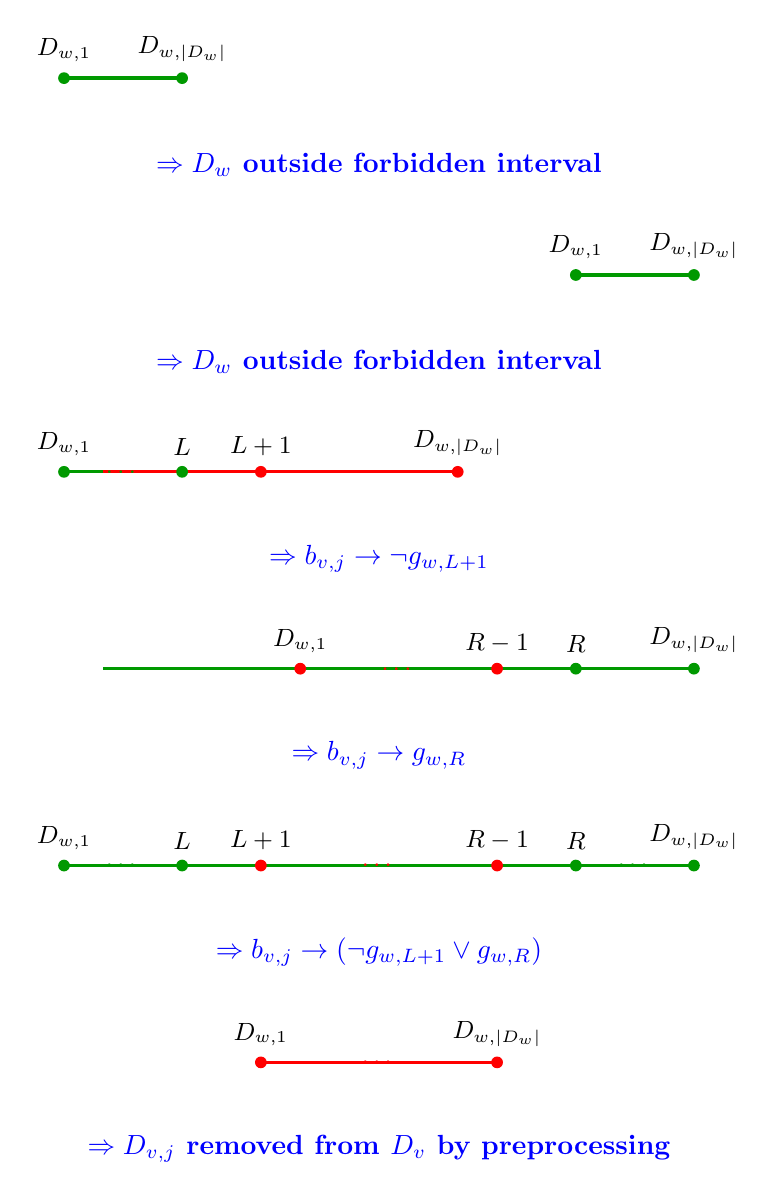
\begin{tikzpicture}[
    font=\small,
    axis/.style={-Latex, thick},
    forbidden/.style={fill=red!8},
    domain_invalid/.style={line width=1.2pt, red},
    domain_valid/.style={line width=1.2pt, green!60!black},
    domain_bound/.style={circle, fill, inner sep=1.5pt}
]

% ==========================================
% Case 1: D_w lies entirely to the left of the forbidden interval
\drawBase{12.5}{Case 1}
\draw[domain_valid] (0.5, 12.8) -- (2.0, 12.8);
\node[domain_bound, green!60!black, label=above:{$D_{w,1}$}] at (0.5, 12.8) {};
\node[green!60!black] at (1.25, 12.8) {$\dots$};
\node[domain_bound, green!60!black, label=above:{$D_{w,|D_w|}$}] at (2.0, 12.8) {};
\node[font=\bfseries, text=blue] at (4.5, 11.7) {$\Rightarrow D_w \text{ outside forbidden interval}$};

% ==========================================
% Case 2: D_w lies entirely to the right of the forbidden interval
\drawBase{10}{Case 2}
\draw[domain_valid] (7.0, 10.3) -- (8.5, 10.3);
\node[domain_bound, green!60!black, label=above:{$D_{w,1}$}] at (7.0, 10.3) {};
\node[green!60!black] at (7.75, 10.3) {$\dots$};
\node[domain_bound, green!60!black, label=above:{$D_{w,|D_w|}$}] at (8.5, 10.3) {};
\node[font=\bfseries, text=blue] at (4.5, 9.2) {$\Rightarrow D_w \text{ outside forbidden interval}$};

% ==========================================
% Case 3: D_w overlaps the forbidden interval on the left
\drawBase{7.5}{Case 3}
\draw[domain_valid] (0.5, 7.8) -- (\fMin, 7.8);
\draw[domain_invalid] (\fMin, 7.8) -- (5.5, 7.8);
\node[domain_bound, green!60!black, label=above:{$D_{w,1}$}] at (0.5, 7.8) {};
\node[green!60!black] at (1.25, 7.8) {$\dots$};
\node[domain_bound, green!60!black, label=above:{$L$}] at (2.0, 7.8) {};
\node[domain_bound, red, label=above:{$L+1$}] at (3.0, 7.8) {};
\node[red] at (4.25, 7.8) {$\dots$};
\node[domain_bound, red, label=above:{$D_{w,|D_w|}$}] at (5.5, 7.8) {};
\node[font=\bfseries, text=blue] at (4.5, 6.7) {$\Rightarrow b_{v,j} \rightarrow \neg g_{w,L+1}$};

% ==========================================
% Case 4: D_w overlaps the forbidden interval on the right
\drawBase{5}{Case 4}
\draw[domain_invalid] (3.5, 5.3) -- (\fMax, 5.3);
\draw[domain_valid] (\fMax, 5.3) -- (8.5, 5.3);
\node[domain_bound, red, label=above:{$D_{w,1}$}] at (3.5, 5.3) {};
\node[red] at (4.75, 5.3) {$\dots$};
\node[domain_bound, red, label=above:{$R-1$}] at (6.0, 5.3) {};
\node[domain_bound, green!60!black, label=above:{$R$}] at (7.0, 5.3) {};
\node[green!60!black] at (7.75, 5.3) {$\dots$};
\node[domain_bound, green!60!black, label=above:{$D_{w,|D_w|}$}] at (8.5, 5.3) {};
\node[font=\bfseries, text=blue] at (4.5, 4.2) {$\Rightarrow b_{v,j} \rightarrow g_{w,R}$};

% ==========================================
% Case 5: D_w extends on both sides of the forbidden interval
\drawBase{2.5}{Case 5}
\draw[domain_valid] (0.5, 2.8) -- (\fMin, 2.8);
\draw[domain_invalid] (\fMin, 2.8) -- (\fMax, 2.8);
\draw[domain_valid] (\fMax, 2.8) -- (8.5, 2.8);
\node[domain_bound, green!60!black, label=above:{$D_{w,1}$}] at (0.5, 2.8) {};
\node[green!60!black] at (1.25, 2.8) {$\dots$};
\node[domain_bound, green!60!black, label=above:{$L$}] at (2.0, 2.8) {};
\node[domain_bound, red, label=above:{$L+1$}] at (3.0, 2.8) {};
\node[red] at (4.5, 2.8) {$\dots$};
\node[domain_bound, red, label=above:{$R-1$}] at (6.0, 2.8) {};
\node[domain_bound, green!60!black, label=above:{$R$}] at (7.0, 2.8) {};
\node[green!60!black] at (7.75, 2.8) {$\dots$};
\node[domain_bound, green!60!black, label=above:{$D_{w,|D_w|}$}] at (8.5, 2.8) {};
\node[font=\bfseries, text=blue] at (4.5, 1.7) {$\Rightarrow b_{v,j} \rightarrow (\neg g_{w,L+1} \lor g_{w,R})$};

% ==========================================
% Case 6: no safe frequency remains; eliminated by preprocessing
\drawBase{0}{Case 6}
\draw[domain_invalid] (3.0, 0.3) -- (6.0, 0.3);
\node[domain_bound, red, label=above:{$D_{w,1}$}] at (3.0, 0.3) {};
\node[red] at (4.5, 0.3) {$\dots$};
\node[domain_bound, red, label=above:{$D_{w,|D_w|}$}] at (6.0, 0.3) {};
\node[font=\bfseries, text=blue] at (4.5, -0.8) {$\Rightarrow D_{v,j}\ \text{removed from }D_v\text{ by preprocessing}$};
\end{tikzpicture}%
}
\caption{Relative positions between the forbidden interval $[D_{v,j}-d_{vw},D_{v,j}+d_{vw}]$ and the domain $D_w$. Red segments denote forbidden values in $D_w$, and green segments denote the remaining values in $D_w$.}
\label{fig:domain_pruning_cases}
\end{figure}
 

\begin{proposition}
\label{prop:pose_correctness}
For the preprocessed domains, POSE ensures that each transmitter is assigned exactly one frequency. More precisely, constraints~\eqref{eq:g_b_connect}--\eqref{eq:g_propagation} are equivalent to the DSE constraint~\eqref{eq:sat_domain}.
Under these constraints,~\eqref{eq:forbid_2} in Case~3,~\eqref{eq:forbid_1} in Case~4, and~\eqref{eq:forbid_3} in Case~5 are satisfied if and only if the assignment to the variables $b$ satisfies the DSE interference constraints~\eqref{eq:sat_ineq}. 
POSE uses the same exact-distance constraints~\eqref{eq:sat_exact} as DSE. 
Therefore, Proposition~\ref{prop:dse_correctness} implies that POSE represents exactly the frequency assignments satisfying constraints~\eqref{eq:ilp_domain},~\eqref{eq:ilp_exact}, and~\eqref{eq:ilp_ineq}.
\end{proposition}
\begin{IEEEproof}
By Lemma~\ref{lem:order_variable_semantics}, every assignment satisfying constraints~\eqref{eq:g_b_connect}--\eqref{eq:g_propagation} has exactly one true variable $b_{v,t}$ for each transmitter $v$. Conversely, suppose that~\eqref{eq:sat_domain} holds and $b_{v,t}$ is the unique true variable for transmitter $v$. Set $g_{v,k}$ to true if and only if $t\ge k$. This assignment satisfies constraints~\eqref{eq:g_b_connect}--\eqref{eq:g_propagation}. Hence, these constraints are equivalent to~\eqref{eq:sat_domain}.

Consider an interference edge $vw\in E_{ineq}$ and an index $j\in\{1,\ldots,|D_v|\}$ such that $b_{v,j}$ is true. Let $b_{w,t}$ be the unique true variable for transmitter $w$. By Lemma~\ref{lem:order_variable_semantics}, $g_{w,k}$ is true if and only if $t\ge k$.
The indices used below are well defined by the corresponding cases described above.

In Case~3, constraint~\eqref{eq:forbid_2} requires $\neg g_{w,L+1}$ because $b_{v,j}$ is true. By Lemma~\ref{lem:order_variable_semantics}, $g_{w,L+1}$ is true if and only if $t\ge L+1$. Therefore, $\neg g_{w,L+1}$ is equivalent to $t\le L$. Since $D_w$ is sorted and $L$ is the largest index satisfying $D_{w,L}<D_{v,j}-d_{vw}$, the selected frequency $D_{w,t}$ lies to the left of the forbidden interval.
For each $k\in\{L+1,\ldots,|D_w|\}$, DSE includes the clause $\neg b_{v,j}\lor\neg b_{w,k}$ in~\eqref{eq:sat_ineq}. Since $b_{v,j}$ is true, these clauses force $b_{w,L+1},\ldots,b_{w,|D_w|}$ to be false. Hence, the unique true variable $b_{w,t}$ must satisfy $t\le L$. DSE therefore imposes the same restriction as~\eqref{eq:forbid_2}.

In Case~4, constraint~\eqref{eq:forbid_1} requires $g_{w,R}$ because $b_{v,j}$ is true. By Lemma~\ref{lem:order_variable_semantics}, this condition is equivalent to $t\ge R$. Since $D_w$ is sorted and $R$ is the smallest index satisfying $D_{w,R}>D_{v,j}+d_{vw}$, the selected frequency $D_{w,t}$ lies to the right of the forbidden interval.
For each $k\in\{1,\ldots,R-1\}$, DSE includes the clause $\neg b_{v,j}\lor\neg b_{w,k}$ in~\eqref{eq:sat_ineq}. Since $b_{v,j}$ is true, these clauses force $b_{w,1},\ldots,b_{w,R-1}$ to be false. Hence, the unique true variable $b_{w,t}$ must satisfy $t\ge R$. DSE therefore imposes the same restriction as~\eqref{eq:forbid_1}.

Case~5 combines the two possibilities established in Cases~3 and~4. When $b_{v,j}$ is true, constraint~\eqref{eq:forbid_3} requires $\neg g_{w,L+1}\lor g_{w,R}$, which is equivalent to $t\le L$ or $t\ge R$. DSE includes the clause $\neg b_{v,j}\lor\neg b_{w,k}$ for each $k\in\{L+1,\ldots,R-1\}$ in~\eqref{eq:sat_ineq}. Since $b_{v,j}$ is true, these clauses force $b_{w,L+1},\ldots,b_{w,R-1}$ to be false. Hence, the unique true variable $b_{w,t}$ must satisfy either $t\le L$ or $t\ge R$. DSE therefore imposes the same restriction as~\eqref{eq:forbid_3}.

In each case, the POSE constraint and the corresponding DSE clauses are equivalent to the same condition on the selected index $t$. Therefore, the equivalence holds in both directions.
Cases~1 and~2 require no additional constraints, while Case~6 cannot occur in the preprocessed domains. If $b_{v,j}$ is false, frequency $D_{v,j}$ is not selected, and neither encoding restricts transmitter $w$ based on this frequency. Therefore, over every interference edge $vw\in E_{ineq}$ and every index $j\in\{1,\ldots,|D_v|\}$, constraints~\eqref{eq:forbid_2},~\eqref{eq:forbid_1}, and~\eqref{eq:forbid_3} exclude exactly the same assignments as~\eqref{eq:sat_ineq}. Together with the equivalence between constraints~\eqref{eq:g_b_connect}--\eqref{eq:g_propagation} and~\eqref{eq:sat_domain}, and the unchanged exact-distance constraints~\eqref{eq:sat_exact}, this establishes the result by Proposition~\ref{prop:dse_correctness}.
\end{IEEEproof}

\subsection{Objective Function Optimization via Incremental SAT}
\label{subsec:incremental_sat}
After the feasibility constraints~\eqref{eq:ilp_domain},~\eqref{eq:ilp_exact}, and~\eqref{eq:ilp_ineq} have been encoded, the remaining task is to minimize the total number of distinct frequencies utilized.
Let $D_m$ denote the frequency value at the $m$-th position of the sorted global domain $D$, where $1 \le m \le N=|D|$.
We introduce Boolean variables $A_m$, where $A_m$ is forced to be $\text{True}$ whenever the frequency $D_m$ is used by at least one transmitter.
The connection between the local assignment variables $b_{v,j}$ and the global frequency-usage variables $A_m$ is expressed by~\eqref{eq:active_link}.
As illustrated in Fig.~\ref{fig:b_to_A_implication}, each selected local assignment $b_{v,j}$ activates the corresponding global usage variable $A_m$, and the objective encoding minimizes the number of active $A_m$ variables.
\begin{align}
    b_{v,j} \rightarrow A_m, \quad \forall v \in V,\; \forall j,m : D_{v,j} = D_m.
    \label{eq:active_link}
\end{align}

\begin{figure}[!htbp]
\centering
\resizebox{\columnwidth}{!}{%
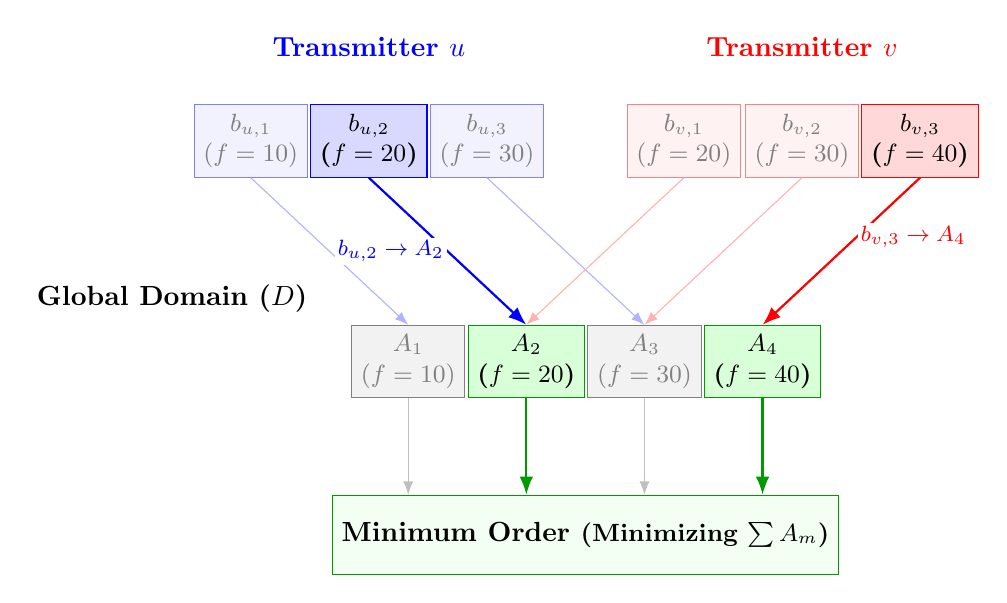
\begin{tikzpicture}[
    node distance = 1.5cm and 1cm,
    var_box/.style = {draw, rectangle, minimum width=1.2cm, minimum height=0.8cm, align=center, font=\small},
    active_u/.style = {var_box, draw=blue, fill=blue!15, font=\small\bfseries},
    inactive_u/.style = {var_box, draw=blue!50, fill=blue!5, text=gray},
    arrow_u/.style = {-Latex, thick, blue},
    active_v/.style = {var_box, draw=red, fill=red!15, font=\small\bfseries},
    inactive_v/.style = {var_box, draw=red!50, fill=red!5, text=gray},
    arrow_v/.style = {-Latex, thick, red},
    active_A/.style = {var_box, draw=green!60!black, fill=green!15, font=\small\bfseries},
    inactive_A/.style = {var_box, draw=gray, fill=gray!10, text=gray},
    arrow_A/.style = {-Latex, thick, green!60!black}
]

% --- Local Domains ---
\node[text=blue] (u_label) at (-1.5, 2.2) {\textbf{Transmitter $u$}};
\node[inactive_u] (xu1) at (-3, 1) {$b_{u,1}$\\($f=10$)};
\node[active_u] (xu2) at (-1.5, 1) {$b_{u,2}$\\($f=20$)}; 
\node[inactive_u] (xu3) at (0, 1) {$b_{u,3}$\\($f=30$)};

\node[text=red] (v_label) at (4, 2.2) {\textbf{Transmitter $v$}};
\node[inactive_v] (xv1) at (2.5, 1) {$b_{v,1}$\\($f=20$)};
\node[inactive_v] (xv2) at (4, 1) {$b_{v,2}$\\($f=30$)};
\node[active_v] (xv3) at (5.5, 1) {$b_{v,3}$\\($f=40$)}; 

% --- Global Frequency Pool ---
\node (global_label) at (-4, -1) {\textbf{Global Domain ($D$)}};
\node[inactive_A] (A1) at (-1, -1.8) {$A_1$\\($f=10$)};
\node[active_A] (A2) at (0.5, -1.8) {$A_2$\\($f=20$)};
\node[inactive_A] (A3) at (2, -1.8) {$A_3$\\($f=30$)};
\node[active_A] (A4) at (3.5, -1.8) {$A_4$\\($f=40$)};

% --- Implications ---
\draw[-Latex, draw=blue!30] (xu1.south) -- (A1.north);
\draw[arrow_u] (xu2.south) -- node[left, pos=0.5, font=\footnotesize, fill=white, inner sep=1pt] {$b_{u,2} \rightarrow A_2$} (A2.north);
\draw[-Latex, draw=blue!30] (xu3.south) -- (A3.north);

\draw[-Latex, draw=red!30] (xv1.south) -- (A2.north);
\draw[-Latex, draw=red!30] (xv2.south) -- (A3.north);
\draw[arrow_v] (xv3.south) -- node[right, pos=0.4, font=\footnotesize, fill=white, inner sep=1pt] {$b_{v,3} \rightarrow A_4$} (A4.north);

% --- Sequential Counter ---
\node[draw=green!60!black, rectangle, minimum width=6cm, minimum height=1cm, fill=green!5, font=\bfseries] (counter) at (1.25, -4) {\textbf{Minimum Order} \small (Minimizing $\sum A_{m}$)};

% Arrows to Counter
\draw[-Latex, draw=gray!50] (A1.south) -- (A1.south |- counter.north);
\draw[arrow_A] (A2.south) -- (A2.south |- counter.north);
\draw[-Latex, draw=gray!50] (A3.south) -- (A3.south |- counter.north);
\draw[arrow_A] (A4.south) -- (A4.south |- counter.north);

\end{tikzpicture}%
}
\caption{Mapping from local assignment variables ($b_{v,j}$) to global frequency-usage variables ($A_m$).}
\label{fig:b_to_A_implication}
\end{figure}
% The optimization of the objective function is performed by a linear search over the number of assigned frequencies. The solver first finds a feasible assignment and uses the number of assigned frequencies as the initial upper bound $UB$. It then searches for a better solution satisfying an At-Most-$k$ constraint with $k=UB-1$. Whenever such a solution is found, $UB$ is updated and the bound is tightened again. 

% These search iterations could be executed as independent SAT calls, where each new value of $k$ requires constructing a new At-Most-$k$ constraint and solving a fresh formula. However, this strategy discards the learned clauses obtained in previous iterations. Therefore, we use the incremental solving mechanism supported by PySAT \cite{imms-sat18,itk-sat24}. In the baseline incremental strategy, denoted as INC, the At-Most-$k$ constraints are handled by \texttt{ITotalizer} \cite{martins2014incremental,Bailleux2003}, which exposes right-hand-side literals that can be passed as assumptions to tighten the cardinality limit across iterations. This allows INC to reuse the same solver instance instead of rebuilding the entire SAT formula for every value of $k$.
% The same optimization pipeline is used by both INC and INCSC, while the difference lies only in the objective encoding and the assumption literal used to enforce each At-Most-$k$ bound. 
% The complete pipeline is summarized in Table~\ref{tab:incremental_pipeline}.
The optimization of the objective function is performed by a linear search over the number of assigned frequencies. The solver first finds a feasible assignment and uses the number of assigned frequencies as the initial upper bound $UB$. It then searches for a better solution satisfying an At-Most-$k$ constraint with $k=UB-1$. Whenever such a solution is found, $UB$ is updated and the bound is tightened again.

These search iterations could be executed as independent SAT calls, where each new value of $k$ requires constructing a new At-Most-$k$ constraint and solving a fresh formula. However, this strategy discards the learned clauses obtained in previous iterations. Therefore, we use the incremental solving mechanism supported by PySAT \cite{imms-sat18,itk-sat24}. The baseline incremental strategy, denoted as INC, handles the At-Most-$k$ constraints by \texttt{ITotalizer} \cite{martins2014incremental,Bailleux2003}. The proposed strategy, denoted as INCSC, uses a Sequential Counter encoding instead. The same optimization pipeline is used by both INC and INCSC. They differ only in the objective encoding and the assumption literal used to enforce each At-Most-$k$ bound. The complete pipeline is summarized in Table~\ref{tab:incremental_pipeline}.

\begin{table}[!t]
\caption{Incremental SAT pipeline for MO-FAP optimization}
\label{tab:incremental_pipeline}
\centering
\begin{tabular}{p{0.18\columnwidth} p{0.74\columnwidth}}
\toprule
\textbf{Input} & Preprocessed MO-FAP instance; selected hard-constraint encoding; selected objective encoding. \\
\midrule
\textit{Step 1} & Construct the hard formula $F$ for the assignment, exact-distance, and interference constraints using DSE~\eqref{eq:sat_domain}--\eqref{eq:sat_ineq} or POSE~\eqref{eq:g_b_connect}--\eqref{eq:g_propagation},~\eqref{eq:forbid_2},~\eqref{eq:forbid_1}, and~\eqref{eq:forbid_3}. \\
\midrule
\textit{Step 2} & Create the global frequency-usage variables $A_m$ for $m=1,\ldots,N$. \\
& Add the usage-linking clauses in~\eqref{eq:active_link} to $F$. \\
\midrule
\textit{Step 3} & Solve $F$. \\
& \textbf{If} $F$ is \texttt{UNSAT}, \textbf{return} \texttt{INF}. \\
& \textbf{If} $F$ is \texttt{SAT}, set $\mathit{best}\leftarrow$ the returned feasible assignment. \\
& Set $UB\leftarrow$ the number of assigned frequencies in $\mathit{best}$. \\
& \textbf{If} $UB=1$, \textbf{return} \texttt{OPT} with $\mathit{best}$ and $UB$. \\
\midrule
\textit{Step 4} & Set $K\leftarrow UB-1$ and build the selected objective encoding for the At-Most-$K$ constraint using \texttt{ITotalizer} for INC or Sequential Counter~\eqref{eq:nsc_1}--\eqref{eq:nsc_7} for INCSC.
\\
\midrule
\textit{Step 5} & \textbf{While} $UB>1$ \textbf{do}: \\
& \quad Set $k\leftarrow UB-1$ and solve $F$ with the corresponding bound. For INC, use the \texttt{ITotalizer} assumption $-\texttt{rhs}[k]$ to enforce At-Most-$k$. For INCSC, use the assumption $\neg S_{N,k+1}$ when \(k<K\). \\
& \quad \textbf{If} the call is \texttt{UNSAT}, \textbf{return} \texttt{OPT} with $\mathit{best}$ and $UB$. \\
& \quad Set $\mathit{best}\leftarrow$ the returned feasible assignment. \\
& \quad Set $UB\leftarrow$ the number of assigned frequencies in $\mathit{best}$. \\
& \textbf{End while}. \\
& \textbf{Return} \texttt{OPT} with $\mathit{best}$ and $UB$. \\
\midrule
\textbf{Output} & \texttt{INF}, or \texttt{OPT} with $\mathit{best}$ as the best feasible assignment and $UB$ as its number of assigned frequencies. \\
\bottomrule
\end{tabular}
\end{table}

In INC, the \texttt{ITotalizer} construction adds the required cardinality clauses to the solver and returns a sequence of output literals, denoted by \texttt{rhs} in PySAT. Each output literal represents a cardinality threshold, so the assumption $-\texttt{rhs}[k]$ enforces the At-Most-$k$ constraint.
During Step~5, the solver searches for a better feasible assignment using at most $k=UB-1$ frequencies. This bound is imposed by passing the assumption $-\texttt{rhs}[k]$ to the solver, which forbids assignments using more than $k$ frequencies. If the call returns \texttt{SAT}, the returned assignment becomes the new $\mathit{best}$, $UB$ is updated to its number of assigned frequencies, and the next iteration repeats the same procedure with the updated value of $UB$.

% Although INC supports learned-clause reuse through assumptions, its Totalizer-based objective encoding introduces considerable structural overhead. 
Although INC supports learned-clause reuse through assumptions, its Totalizer-based objective encoding introduces more auxiliary structure than the Sequential Counter encoding.
To reduce this overhead, INCSC keeps the same assumptions-based optimization loop as INC but replaces the Totalizer with a Sequential Counter encoding~\cite{Sinz2005}. 
For the variables $A_1,\dots,A_N$, indexed by the sorted global domain $D$, INCSC introduces auxiliary variables $S_{i,c}$, where $1 \le i \le N$ and $1 \le c \le \min(i,K)$.
The variable $S_{i,c}$ is true if and only if at least $c$ variables among $A_1,\dots,A_i$ are true. Equivalently, each prefix state $S_i$ is a vector of $\min(i,K)$ bits, $S_i=(S_{i,1},\dots,S_{i,\min(i,K)})$: $S_1$ has one bit, $S_2$ has two bits, and for $i \ge K$, $S_i$ has $K$ bits. This semantics is enforced by the constraints in~\eqref{eq:nsc_1}--\eqref{eq:nsc_7}. 
% As a result, INCSC reduces the objective encoding to $\mathcal{O}(NK)$ auxiliary variables and clauses, compared with the $\mathcal{O}(N \log N)$ auxiliary variables and $\mathcal{O}(N^2)$ clauses required by INC.
As a result, INCSC uses $\mathcal{O}(NK)$ auxiliary variables and clauses, compared with the $\mathcal{O}(N \log N)$ auxiliary variables and $\mathcal{O}(N^2)$ clauses required by INC.
\begin{align}
    & \bigwedge_{i=1}^{N} \left( A_i \rightarrow S_{i,1} \right) \label{eq:nsc_1} \\
    & \bigwedge_{i=2}^{N} \;\bigwedge_{c=1}^{\min(i-1,K)} \left( S_{i-1,c} \rightarrow S_{i,c} \right) \label{eq:nsc_2} \\
    & \bigwedge_{i=2}^{N} \;\bigwedge_{c=2}^{\min(i,K)} \left( A_i \land S_{i-1,c-1} \rightarrow S_{i,c} \right) \label{eq:nsc_3} \\
    & \bigwedge_{i=2}^{N} \;\bigwedge_{c=1}^{\min(i-1,K)} \left( \neg A_i \land \neg S_{i-1,c} \rightarrow \neg S_{i,c} \right) \label{eq:nsc_4} \\
    & \bigwedge_{i=1}^{K} \left( \neg A_i \rightarrow \neg S_{i,i} \right) \label{eq:nsc_5} \\
    & \bigwedge_{i=2}^{N} \;\bigwedge_{c=2}^{\min(i,K)} \left( \neg S_{i-1,c-1} \rightarrow \neg S_{i,c} \right) \label{eq:nsc_6} \\
    & \bigwedge_{i=K+1}^{N} \left( A_i \rightarrow \neg S_{i-1,K} \right) \label{eq:nsc_7}
\end{align}

% After the Sequential Counter encoding in \eqref{eq:nsc_1}--\eqref{eq:nsc_7} is built, it enforces the initial bound $K=UB-1$, while any tighter At-Most-$k$ bound with $k<K$ is enforced by the single assumption $\neg S_{N,k+1}$.
% Since $S_{N,k+1}$ represents that at least $k+1$ frequencies are active, assuming $\neg S_{N,k+1}$ forces the solution to use at most $k$ frequencies. 
% % Thus, each iteration only changes the assumption literal, while the objective encoding remains unchanged.
% This design is particularly effective for incremental SAT solving, as each iteration introduces a unary clause, implemented as an assumption over an auxiliary variable generated by the Sequential Counter encoding, enabling efficient reuse of learned clauses.
In Step~4 of Table~\ref{tab:incremental_pipeline}, the Sequential Counter encoding in~\eqref{eq:nsc_1}--\eqref{eq:nsc_7} is built once for the initial bound $K=UB-1$. In Step~5, any tighter At-Most-$k$ bound with $k<K$ is enforced by the single assumption $\neg S_{N,k+1}$. Since $S_{N,k+1}$ represents that at least $k+1$ frequencies are active, assuming $\neg S_{N,k+1}$ forces the solution to use at most $k$ frequencies. Thus, each iteration changes only the assumption literal, while the Sequential Counter encoding remains unchanged and the solver can reuse learned clauses. For both INC and INCSC, once the At-Most-$k$ constraint is enforced by the corresponding assumption, the same stopping condition applies. Its correctness is formalized in Proposition~\ref{prop:incremental_optimality}.
\begin{proposition}
\label{prop:incremental_optimality}
Let $UB>1$ denote the number of distinct frequencies used by the current best feasible assignment. 
If the next SAT call enforces the At-Most-$k$ constraint with $k=UB-1$ over the global frequency-usage variables $A_m$ and returns \texttt{UNSAT}, then the current value $UB$ is globally optimal.
\end{proposition}
\begin{IEEEproof}
By the definition of $b_{v,j}$ and by~\eqref{eq:active_link}, if transmitter $v$ is assigned frequency $D_{v,j}=D_m$, then $b_{v,j}$ is true and the corresponding variable $A_m$ is forced to be true.
Thus, every used frequency has its corresponding variable $A_m$ set to true.
Therefore, any model satisfying an At-Most-$k$ constraint over the variables $A_m$ uses at most $k$ distinct frequencies.
Any feasible assignment using at most $k$ distinct frequencies can set at most $k$ variables $A_m$ to true, namely those corresponding to the used frequencies. Therefore, it satisfies both~\eqref{eq:active_link} and the At-Most-$k$ constraint, so the bounded formula does not incorrectly exclude such an assignment.
Consequently, if the SAT call enforcing the At-Most-$k$ constraint with $k=UB-1$ returns \texttt{UNSAT}, then no feasible assignment exists that uses at most $UB-1$ distinct frequencies.
This means that every feasible assignment uses at least $UB$ distinct frequencies. On the other hand, the current best assignment is feasible and uses exactly $UB$ distinct frequencies. Therefore, $UB$ is the minimum possible number of distinct frequencies and is globally optimal.
\end{IEEEproof}


\section{Experiments}
\label{sec:exp}
\subsection{Experimental Setup}
% All experiments were conducted on a workstation equipped with an Intel Core i7-10850H processor and 16 GB of RAM, running the Ubuntu 24.04.3 LTS operating system. The SAT solving processes were executed using the CaDiCaL solver (version 1.9.5) via the \texttt{PySAT} toolkit \cite{imms-sat18,itk-sat24}. To strictly control and accurately monitor the resource consumption of the algorithms, we integrated the \texttt{runlim} tool \texttt{\url{https://github.com/arminbiere/runlim/}}. 
% For each instance, the system imposed strict computational boundaries: a maximum execution time of 600 seconds and a maximum allocated memory of 14,000 MB. Any process exceeding the time threshold was forcefully terminated and recorded as a Timeout (TO).

% The evaluations were performed on two standard benchmark datasets, CALMA and DUTtest, which have been widely verified in previous studies (archived in the FAP web database \texttt{\url{https://fap.zib.de/}}).
% For the CALMA dataset, in addition to the instances originally designed for the MO-FAP, we expanded the evaluation space by reformulating the objective functions of all remaining CELAR and GRAPH instances into the MO-FAP format. This reformulation strategy is specifically intended to rigorously assess the solver's stability and pruning capabilities when dealing with inherently infeasible instances. Furthermore, to diversify the experimental dataset and provide a comprehensive evaluation, the DUTtest benchmark also available from the aforementioned database was incorporated into our experiments. Detailed structural characteristics of all individual benchmark instances, including the specific number of transmitters ($|V|$) and bidirectional and interference constraints ($|E|$), are fully documented and publicly available on the FAP website.

% To comprehensively and objectively evaluate the model's performance, a multi-dimensional benchmarking framework was established. First, POSE was directly compared against DSE to highlight the efficacy of the order-based interference formulation. Next, the overall strength of the proposed system was benchmarked against leading commercial optimization software, specifically the Mixed-Integer Programming (MIP) and Constraint Programming (CP) solvers provided by Gurobi (v12.0.3) \texttt{\url{https://www.gurobi.com}} and IBM ILOG CPLEX (v12.1.1) \texttt{\url{https://www.ibm.com/products/ilog-cplex-optimization-studio}}. For computational efficiency in these baseline solvers, the interference constraints~\eqref{eq:ilp_exact} and~\eqref{eq:ilp_ineq} are programmatically implemented using mathematically equivalent summations.
% The complete source code and datasets for these experiments are publicly available at: \texttt{\url{https://github.com/dev2points/Min-Order-Frequency-Assignment-Problem}}.

% To standardize the presentation of the experimental results, we adopt a strict naming convention for the algorithmic configurations. The problem encoding models are denoted as \textbf{DSE} (Direct SAT Encoding) and \textbf{POSE} (Proposed Order-based SAT Encoding). These encodings are coupled with one of two incremental optimization strategies: \textbf{INC}, the baseline approach utilizing the \texttt{ITotalizer} abstraction from the \texttt{PySAT} library, or \textbf{INCSC}, our proposed approach utilizing the Sequential Counter. A complete SAT-based solving framework is explicitly defined by concatenating the encoding model with the optimization strategy. We systematically evaluate three specific SAT configurations: \textbf{POSE+INCSC} represents our ultimate proposed framework, whereas \textbf{POSE+INC} and \textbf{DSE+INCSC} serve as internal baselines for rigorous ablation analysis. Finally, the state-of-the-art commercial exact solvers are strictly referred to as \textbf{Gurobi}, \textbf{CPLEX-MIP}, and \textbf{CPLEX-CP}.
All experiments were conducted on a workstation with an Intel Core i7-10850H processor and 16 GB RAM running Ubuntu 24.04.3 LTS. The SAT-based methods were implemented with CaDiCaL (v1.9.5) through \texttt{PySAT} \cite{imms-sat18,itk-sat24}. Each run was executed under \texttt{runlim} with a time limit of 600 seconds and a memory limit of 14,000 MB.

The evaluation was performed on the standard CALMA and DUTtest benchmarks from the FAP web database \texttt{\url{https://fap.zib.de/}}. In addition to the native MO-FAP instances, we also reformulated CELAR and GRAPH instances into the MO-FAP objective. For these reformulated instances, the original constraints are kept unchanged, and only the objective is set to Minimum Order. Table~\ref{tab:benchmark_instances} summarizes the benchmark instances used in the experiments, where $|V|$ and $|E|$ denote the number of transmitters and distance constraints, respectively.
% The implementation and benchmark data are publicly available at \texttt{\url{https://github.com/dev2points/Min-Order-Frequency-Assignment-Problem}}.
\begin{table}[!htbp]
\centering
\caption{Benchmark instances used in the experiments}
\label{tab:benchmark_instances}
\scriptsize
\setlength{\tabcolsep}{3pt}
\renewcommand{\arraystretch}{1.0}
\begin{tabular}{@{}llp{0.29\columnwidth}rr@{}}
\toprule
\textbf{Instance} & \textbf{Original Name} & \textbf{Original Objective} & $|V|$ & $|E|$ \\
\midrule
C01 & CELAR 01 & Minimum Order & 916 & 5548 \\
C02 & CELAR 02 & Minimum Order & 200 & 1235 \\
C03 & CELAR 03 & Minimum Order & 400 & 2760 \\
C04 & CELAR 04 & Minimum Order & 680 & 3967 \\
C05 & CELAR 05 & Minimum Span & 400 & 2598 \\
C06 & CELAR 06 & Minimum Interference & 200 & 1322 \\
C07 & CELAR 07 & Minimum Interference & 400 & 2865 \\
C08 & CELAR 08 & Minimum Interference & 916 & 5744 \\
C09 & CELAR 09 & Minimum Interference & 680 & 4103 \\
C10 & CELAR 10 & Minimum Interference & 680 & 4103 \\
C11 & CELAR 11 & Minimum Order & 680 & 4103 \\
G01 & GRAPH 01 & Minimum Order & 200 & 1134 \\
G02 & GRAPH 02 & Minimum Order & 400 & 2245 \\
G03 & GRAPH 03 & Minimum Span & 200 & 1134 \\
G04 & GRAPH 04 & Minimum Span & 400 & 2244 \\
G05 & GRAPH 05 & Minimum Interference & 200 & 1134 \\
G06 & GRAPH 06 & Minimum Interference & 400 & 2170 \\
G07 & GRAPH 07 & Minimum Interference & 400 & 2170 \\
G08 & GRAPH 08 & Minimum Order & 680 & 3757 \\
G09 & GRAPH 09 & Minimum Order & 916 & 5246 \\
G10 & GRAPH 10 & Minimum Span & 680 & 3907 \\
G11 & GRAPH 11 & Minimum Interference & 680 & 3757 \\
G12 & GRAPH 12 & Minimum Interference & 680 & 4017 \\
G13 & GRAPH 13 & Minimum Interference & 916 & 5273 \\
G14 & GRAPH 14 & Minimum Order & 916 & 4638 \\
T2.1 & TUD200.1 & Minimum Order & 200 & 1171 \\
T2.2 & TUD200.2 & Minimum Order & 200 & 1143 \\
T2.3 & TUD200.3 & Minimum Order & 200 & 1160 \\
T2.4 & TUD200.4 & Minimum Order/Span & 200 & 1142 \\
T2.5 & TUD200.5 & Minimum Interference & 200 & 1125 \\
T9.1 & TUD916.1 & Minimum Order & 916 & 5177 \\
T9.2 & TUD916.2 & Minimum Order & 916 & 5173 \\
T9.3 & TUD916.3 & Minimum Order & 916 & 5262 \\
T9.4 & TUD916.4 & Minimum Order/Span & 916 & 5183 \\
T9.5 & TUD916.5 & Minimum Interference & 916 & 5213 \\
\bottomrule
\end{tabular}
\end{table}
% For clarity, we denote the two SAT encodings as \textbf{DSE} (Direct SAT Encoding) and \textbf{POSE} (Proposed Order-based SAT Encoding). We also consider two incremental optimization strategies: \textbf{INC}, which employs \texttt{ITotalizer} for incremental cardinality constraints, and \textbf{INCSC}, which utilizes the Sequential Counter encoding described in Section~\ref{subsec:incremental_sat}. A complete solver configuration is named by combining one encoding and one optimization strategy; therefore, \textbf{POSE+INCSC} denotes the proposed method, while \textbf{POSE+INC} and \textbf{DSE+INCSC} are used as ablation baselines.
% The proposed framework is further compared against Gurobi, CPLEX-CP, and CPLEX-MIP.
% The proposed framework is further compared against three commercial exact solvers: Gurobi (v12.0.3), CPLEX-CP, and CPLEX-MIP (IBM ILOG CPLEX Optimization Studio v12.1.1), where CPLEX-CP and CPLEX-MIP denote the constraint programming and mixed-integer programming modes of CPLEX, respectively.
% The SAT-based methods differ in terms of how the feasibility constraints and the objective function are handled. For the feasibility constraints, DSE and POSE correspond to the encodings described in Sections~\ref{subsec:sat_encoding} and~\ref{subsec:order_encoding}, respectively. CARD keeps the same modeling target as DSE but replaces the SAT encodings of~\eqref{eq:sat_domain} and~\eqref{eq:sat_ineq}, which correspond to~\eqref{eq:ilp_domain} and~\eqref{eq:ilp_ineq}, by PySAT cardinality encodings. For the objective function, INC and INCSC correspond to the incremental SAT strategies described in Section~\ref{subsec:incremental_sat}. The proposed framework is further compared against Gurobi, CPLEX-CP, CPLEX-MIP, CP-SAT, and MaxSAT+POSE. Here, CPLEX-CP and CPLEX-MIP denote the constraint programming and mixed-integer programming models of CPLEX, respectively. Table~\ref{tab:method_notation} summarizes the method names used in the experimental results.
\begin{table}[!htbp]
\centering
\caption{Methods compared in the experiments}
\label{tab:method_notation}
\scriptsize
\setlength{\tabcolsep}{3pt}
\renewcommand{\arraystretch}{1.05}
\begin{tabular}{@{}p{0.32\columnwidth}p{0.63\columnwidth}@{}}
\toprule
\textbf{Method} & \textbf{Description} \\
\midrule
\multicolumn{2}{@{}l}{\textit{SAT encodings and objective strategies}} \\
DSE & Direct SAT encoding with pairwise interference clauses. \\
CARD-Seq & Cardinality-based SAT encoding for~\eqref{eq:sat_domain} and~\eqref{eq:sat_ineq} using PySAT Sequential Counter encodings. \\
POSE & Proposed order-based SAT encoding. \\
INC & Incremental SAT optimization using \texttt{ITotalizer}. \\
INCSC & Incremental SAT optimization using Sequential Counter. \\
MaxSAT-RC2 & MaxSAT optimization using PySAT RC2 with hard feasibility clauses and unit soft clauses over the global frequency-usage variables $A_m$. \\
\midrule
\multicolumn{2}{@{}l}{\textit{Main SAT configuration}} \\
POSE+INCSC & POSE combined with INCSC. \\
\midrule
\multicolumn{2}{@{}l}{\textit{Feasibility-encoding comparison with INCSC}} \\
POSE+INCSC & POSE combined with INCSC. \\
DSE+INCSC & DSE combined with INCSC. \\
CARD-Seq+INCSC & CARD-Seq combined with INCSC. \\
\midrule
\multicolumn{2}{@{}l}{\textit{Objective-optimization comparison with POSE}} \\
POSE+INCSC & POSE combined with INCSC. \\
POSE+INC & POSE combined with INC. \\
POSE+MaxSAT-RC2 & POSE combined with MaxSAT-RC2. \\
\midrule
\multicolumn{2}{@{}l}{\textit{Baseline methods}} \\
Gurobi & Gurobi MIP solver (v12.0.3). \\
CPLEX-CP & CP model in CPLEX Optimization Studio (v12.1.1). \\
CPLEX-MIP & MIP model in CPLEX Optimization Studio (v12.1.1). \\
CP-SAT & CP-SAT solver in Google OR-Tools (v9.15.6755). \\
\bottomrule
\end{tabular}
\end{table}

Table~\ref{tab:method_notation} summarizes the method names used in the experimental results.
The SAT-based methods differ in terms of how the feasibility constraints and the objective function are handled. For the feasibility constraints, DSE and POSE correspond to the encodings described in Sections~\ref{subsec:sat_encoding} and~\ref{subsec:order_encoding}, respectively.
In addition to DSE and POSE, CARD denotes cardinality-based SAT encodings that encode~\eqref{eq:sat_domain} as an Exactly-One constraint and encode~\eqref{eq:sat_ineq} through At-Most-One constraints using PySAT.
Among the evaluated CARD variants, including Totalizer (CARD-Totalizer) and Cardinality Network (CARD-CardNet) encodings, Sequential Counter (CARD-Seq) is selected as the representative CARD baseline in the main results. The detailed results for CARD-Totalizer and CARD-CardNet are reported in Table~\ref{tab:appendix_sat_core_preprocess}.

% For the objective function, INC and INCSC correspond to the incremental SAT strategies described in Section~\ref{subsec:incremental_sat}. In addition to INC and INCSC, MaxSAT is included as a baseline for objective-function optimization. In this baseline, the feasibility constraints and the usage-linking clauses~\eqref{eq:active_link} are added as hard clauses, while each global frequency-usage variable $A_m$ contributes a unit soft clause $\neg A_m$ with weight one.
For the objective function, INC and INCSC correspond to the incremental SAT strategies described in Section~\ref{subsec:incremental_sat}. 
MaxSAT-RC2 is included in the main results as an objective-optimization baseline.
In this MaxSAT-RC2 formulation, the feasibility constraints and the usage-linking clauses~\eqref{eq:active_link} are added as hard clauses, while each global frequency-usage variable $A_m$ contributes a unit soft clause $\neg A_m$ with weight one. 
Results for an additional MaxSAT solver, EvalMaxSAT (POSE+EvalMaxSAT), are reported in Table~\ref{tab:appendix_solver_baselines_preprocess}.

The proposed framework is further compared against several commonly used optimization solvers, including Gurobi, CPLEX-CP, CPLEX-MIP, and OR-Tools CP-SAT.
All methods were also run under the same external limits of 600 seconds and 14,000 MB memory using \texttt{runlim}. Gurobi, CPLEX-CP, and OR-Tools CP-SAT used their default solver configurations. CPLEX-MIP also used its standard solver configuration, except that zero MIP gap was set to require an exact optimality certificate and its built-in presolve routine was enabled.

The outcome of each evaluated method on each benchmark instance is reported using one of three final statuses. \texttt{OPT} denotes that optimality is certified, \texttt{INF} denotes that the instance is proven infeasible, and \texttt{TO} denotes that the run reaches the 600-second time limit without a certificate. When cumulative solving time is reported, each \texttt{TO} run is counted as 600 seconds. Details on the benchmark data, experimental results, and source code are provided in the Data and Code Availability statement.

\subsection{Evaluation of Domain Preprocessing}
% Problem reduction through preprocessing is highly effective for reducing the size of the initial problem formulation. The empirical data, visually summarized in the scatter plot in Fig.~\ref{fig:preprocess_scatter}, reveals that preprocessing acts as a powerful catalyst for both the SAT-based models and commercial solvers. Specifically, for the proposed POSE+INCSC, pruning invalid frequency domains successfully accelerates the search process in 80.00\% of the overall instances (28 out of 35). Moreover, it effectively rescues CPLEX-MIP and CPLEX-CP from severe time limitations in 2 and 1 highly constrained instances, respectively. 
% The most profound impact, however, is observed in the 13 inherently infeasible (\texttt{INF}) instances, where the preprocessing technique accelerates the execution time in 100\% of the cases for POSE+INCSC, DSE+INCSC, Gurobi, and CPLEX-MIP. Many instances in the standard benchmark datasets were originally designed for other objectives (e.g., MS-FAP or MI-FAP) and have thus been reformulated to evaluate the MO-FAP. Because these original instances were already strictly constrained for their initial targets, the margin for further minimizing the number of assigned frequencies is extremely narrow. Nevertheless, the core purpose of utilizing these modified instances is to rigorously test the exact solvers' capability in search space pruning and proving infeasibility (\texttt{UNSAT}). Powered by the domain preprocessing technique combined with the SAT's unit propagation mechanism, the proposed model demonstrates an outstanding ability to certify the \texttt{UNSAT} status almost instantaneously. As observed in Fig.~\ref{fig:preprocess_scatter}, the vast majority of data points gravitate toward the region below the $y=x$ boundary, representing a consistent performance gain across a wide range of problem complexities.
% Domain preprocessing substantially reduces the initial formulation. As shown in Fig.~\ref{fig:preprocess_scatter}, it speeds up POSE+INCSC on 28 of the 35 instances and also mitigates severe time degradation for CPLEX-MIP and CPLEX-CP on several hard cases. The effect is especially clear on the 13 infeasible (\texttt{INF}) instances, where preprocessing improves solving time in every case for POSE+INCSC, DSE+INCSC, Gurobi, and CPLEX-MIP. Many of these instances were reformulated from other FAP objectives, making them suitable for evaluating search-space pruning and infeasibility certification. 
% Most points in Fig.~\ref{fig:preprocess_scatter} lie below the $y=x$ line, indicating that preprocessing consistently reduces solving time across a broad range of instances, with the clearest gains observed on the infeasible (\texttt{INF}) cases.
\begin{figure}[!h]
    \centering
    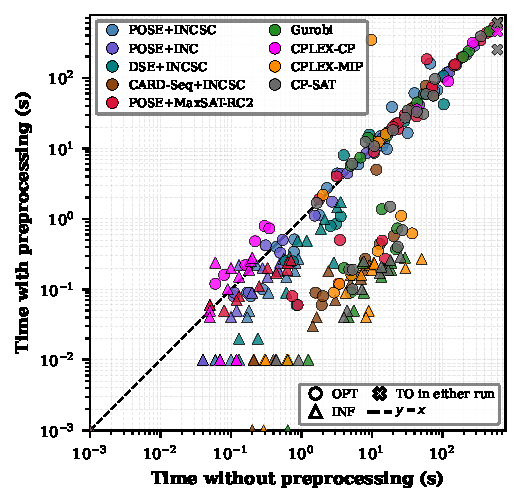
\includegraphics[width=0.7\columnwidth]{image/iv_b_runtime_scatter_by_solver.pdf} 
    \caption{Solving time with and without domain preprocessing on 35 benchmark instances.}
    \label{fig:preprocess_scatter}
\end{figure}
% This experiment evaluates the contribution of domain preprocessing to the solving process. As shown in Fig.~\ref{fig:preprocess_scatter}, POSE+INCSC is faster with preprocessing on 28 of the 35 instances. The same comparison is also reported for POSE+INC, DSE+INCSC, CARD-Seq+INCSC, POSE+MaxSAT-RC2, Gurobi, CPLEX-MIP, CPLEX-CP, and CP-SAT.
% This experiment evaluates the contribution of domain preprocessing to the solving process. As shown in Fig.~\ref{fig:preprocess_scatter}, POSE+\allowbreak INCSC is faster with preprocessing on 28 of the 35 instances. The same comparison is also reported for POSE+\allowbreak INC, DSE+\allowbreak INCSC, CARD-\allowbreak Seq+\allowbreak INCSC, POSE+\allowbreak MaxSAT-\allowbreak RC2, Gurobi, CPLEX-\allowbreak MIP, CPLEX-\allowbreak CP, and CP-\allowbreak SAT.
% The effect is particularly visible on the 13 infeasible (\texttt{INF}) instances, where preprocessing reduces the time required to prove infeasibility for both POSE+INCSC and DSE+INCSC. For Gurobi and CPLEX-MIP, it reduces the solving time on all infeasible instances. Overall, most points in Fig.~\ref{fig:preprocess_scatter} lie below the $y=x$ line, indicating that preprocessing is beneficial in this evaluation. A few points lie above the diagonal, but most of these points remain close to it, indicating that the slowdown is usually limited when preprocessing is not beneficial.

% This experiment evaluates how domain preprocessing affects solving time and infeasibility certification. As shown in Fig.~\ref{fig:preprocess_scatter}, many points in the upper-left and middle regions lie close to the $y=x$ line, indicating that preprocessing has a limited effect on those runs. In contrast, the points in the lower-right region are farther below the diagonal, showing larger reductions in solving time when preprocessing is enabled. This pattern is especially clear for infeasible (\texttt{INF}) instances, whose markers frequently move to the low-runtime region after preprocessing. For POSE+INCSC, preprocessing reduces solving time on 28 of the 35 instances. The same comparison is also reported for POSE+INC, DSE+INCSC, CARD-Seq+INCSC, POSE+MaxSAT-RC2, Gurobi, CPLEX-MIP, CPLEX-CP, and CP-SAT.
This experiment examines whether domain preprocessing reduces solving time for the evaluated methods shown in Fig.~\ref{fig:preprocess_scatter}. 
Overall, preprocessing improves solving time for most of the evaluated methods on a substantial subset of instances, with the clearest effect observed on infeasible (\texttt{INF}) instances. For POSE+INCSC, enabling preprocessing reduces solving time on 28 of the 35 instances. 
In Fig.~\ref{fig:preprocess_scatter}, points close to the $y=x$ line correspond to runs where preprocessing has limited effect, whereas points below the diagonal indicate faster solving after preprocessing. The largest reductions are mainly associated with infeasible instances, where inconsistent domain values can be removed before the main solving process.

\subsection{Evaluation of the Proposed Order-Based SAT Encoding}

\begin{table}[!htbp]
\centering
\caption{Number of variables and clauses in the SAT encodings of the assignment, exact-distance, and interference constraints for instances not eliminated by preprocessing.}
\label{tab:hard_encoding_full}
\scriptsize
\setlength{\tabcolsep}{2.2pt}
\renewcommand{\arraystretch}{1.0}
\begin{tabular}{@{}lrrrrrrrrrr@{}}
\toprule
\multirow{2}{*}{\textbf{Inst.}} & \multicolumn{5}{c}{\textbf{Variables}} & \multicolumn{5}{c}{\textbf{Clauses}} \\
\cmidrule(lr){2-6}\cmidrule(lr){7-11}
& \textbf{DSE} & \textbf{POSE} & \textbf{P/D} & \textbf{CARD} & \textbf{C/D} & \textbf{DSE} & \textbf{POSE} & \textbf{P/D} & \textbf{CARD} & \textbf{C/D} \\
\midrule
C01 & \textbf{36,200} & 72,400 & 200 & 692,321 & 1912 & 1,446,348 & \textbf{355,326} & 25 & 1,982,888 & 137 \\
C02 & \textbf{8,004} & 16,008 & 200 & 181,777 & 2271 & 349,519 & \textbf{82,133} & 23 & 522,669 & 150 \\
C03 & \textbf{15,892} & 31,784 & 200 & 362,247 & 2279 & 702,647 & \textbf{173,390} & 25 & 1,047,531 & 149 \\
C04 & \textbf{1,960} & 3,920 & 200 & 5,783 & 295 & \textbf{10,472} & 11,930 & 114 & 12,729 & 122 \\
C05 & \textbf{3,722} & 7,444 & 200 & 73,726 & 1981 & 107,224 & \textbf{26,565} & 25 & 205,588 & 192 \\
C11 & \textbf{26,856} & 53,712 & 200 & 548,487 & 2042 & 1,105,353 & \textbf{268,996} & 24 & 1,573,495 & 142 \\
G01 & \textbf{6,920} & 13,840 & 200 & 71,739 & 1037 & 206,786 & \textbf{62,950} & 30 & 196,572 & 95 \\
G02 & \textbf{14,624} & 29,248 & 200 & 172,559 & 1180 & 475,829 & \textbf{139,391} & 29 & 478,208 & 100 \\
G03 & \textbf{7,480} & 14,960 & 200 & 463,875 & 6202 & 598,543 & \textbf{71,704} & 12 & 1,341,243 & 224 \\
G04 & \textbf{14,816} & 29,632 & 200 & 904,601 & 6106 & 1,168,001 & \textbf{140,881} & 12 & 2,615,266 & 224 \\
G08 & \textbf{25,628} & 51,256 & 200 & 389,284 & 1519 & 906,033 & \textbf{236,932} & 26 & 1,079,747 & 119 \\
G09 & \textbf{36,092} & 72,184 & 200 & 573,735 & 1590 & 1,299,985 & \textbf{352,970} & 27 & 1,599,202 & 123 \\
G10 & \textbf{26,594} & 53,188 & 200 & 1,781,951 & 6701 & 2,273,085 & \textbf{256,868} & 11 & 5,163,511 & 227 \\
G14 & \textbf{36,716} & 73,432 & 200 & 462,509 & 1260 & 1,204,487 & \textbf{334,704} & 28 & 1,269,682 & 105 \\
T2.1 & \textbf{7,986} & 15,972 & 200 & 173,596 & 2174 & 339,265 & \textbf{78,025} & 23 & 493,586 & 145 \\
T2.2 & \textbf{200} & 400 & 200 & \textbf{200} & 100 & \textbf{300} & 1,286 & 429 & \textbf{300} & 100 \\
T2.3 & \textbf{7,066} & 14,132 & 200 & 153,407 & 2171 & 288,705 & \textbf{66,557} & 23 & 433,731 & 150 \\
T2.4 & \textbf{624} & 1,248 & 200 & 5,275 & 845 & 9,049 & \textbf{4,050} & 45 & 13,974 & 154 \\
T9.1 & \textbf{33,572} & 67,144 & 200 & 705,399 & 2101 & 1,380,601 & \textbf{306,313} & 22 & 2,000,264 & 145 \\
T9.2 & \textbf{1,180} & 2,360 & 200 & 1,454 & 123 & 2,490 & 7,147 & 287 & \textbf{2,312} & 93 \\
T9.3 & \textbf{34,386} & 68,772 & 200 & 756,304 & 2199 & 1,443,466 & \textbf{329,553} & 23 & 2,144,292 & 149 \\
T9.4 & \textbf{2,886} & 5,772 & 200 & 9,100 & 315 & \textbf{15,888} & 16,813 & 106 & 20,280 & 128 \\
\midrule
\multicolumn{11}{@{}l}{\scriptsize P/D and C/D are percentages relative to DSE.} \\
\bottomrule
\end{tabular}
\end{table}

\begin{table}[!htbp]
\centering
\caption{Number of benchmark instances certified by each SAT encoding after preprocessing.}
\label{tab:pose_encoding_certification}
\footnotesize
\setlength{\tabcolsep}{2.2pt}
\begin{tabular}{lrrrrr}
\toprule
Method & \#OPT & \#INF & \#TO & \#Certified & Total time (s) \\
\midrule
POSE+INCSC & 22 & 13 & 0 & 35/35 & 599.94 \\
DSE+INCSC & 13 & 13 & 9 & 26/35 & 5723.34 \\
CARD-Seq+INCSC & 13 & 13 & 9 & 26/35 & 5786.33 \\
\bottomrule
\end{tabular}
\end{table}



\begin{figure}[!htbp]
\centering
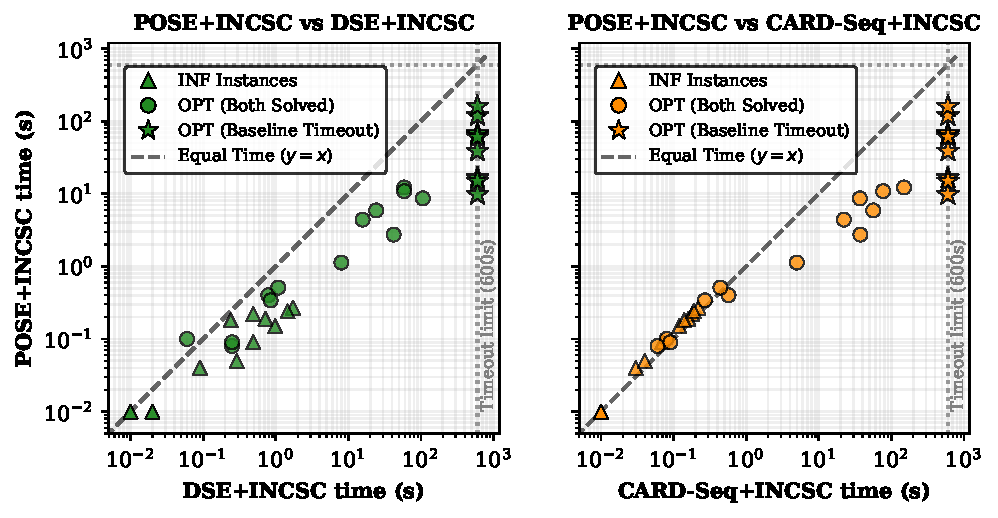
\includegraphics[width=\columnwidth]{image/pose_encoding_pair_scatter.pdf}
\caption{Comparison of solving time between POSE+INCSC and two SAT encoding baselines, DSE+INCSC and CARD-Seq+INCSC, on 35 benchmark instances.}
\label{fig:pose_encoding_pair_scatter}
\end{figure}



% % This experiment evaluates the computational performance of POSE against DSE baseline, with both utilizing domain preprocessing and the \textit{INCSC} strategy. 
% This experiment compares POSE against DSE under the same domain preprocessing and \textit{INCSC} strategy.
% % The empirical data strongly validates the comprehensive superiority of POSE over the direct encoding approach in terms of both execution time and overall convergence capability. 
% % In particular, POSE successfully solves and mathematically certifies all 35 instances within the 600-second limit, achieving an absolute success rate of 100\%. 
% POSE successfully solves and mathematically certifies all 35 instances within the 600-second limit.
% As clearly depicted by the distribution of data points falling entirely below the $y=x$ reference line, the proposed POSE model consistently operates at a higher speed than the baseline.
% % Overall, the structural efficiency of POSE reduces the cumulative execution time across all 35 instances from 5723.34 seconds to merely 599.94 seconds, representing an aggregate computational savings of approximately 89.52\%.
% Overall, the structural efficiency of POSE reduces the penalized cumulative execution time across all 35 instances from 5723.34 seconds (which includes the 600-second timeout penalties for the 9 uncertified instances) to merely 599.94 seconds, representing an aggregate computational savings of approximately 89.52\%.

% The structural power of the proposed encoding is further underscored by inherently infeasible instances (\texttt{INF}). To conclusively certify an \texttt{INF} status (i.e., \texttt{UNSAT}), the exact solver is compelled to exhaustively traverse and prune the entire search space. The results demonstrate that POSE reaches the \texttt{UNSAT} conclusion strictly faster than, or equivalently to, DSE in 100\% of these test cases. This consistent disparity serves as robust evidence for the efficacy of the proposed order-based interference encoding, demonstrating that the established auxiliary variables $g$ effectively accelerate the unit propagation process without introducing computational overhead.
This experiment evaluates the effect of the SAT encoding used for the assignment, exact-distance, and interference constraints while keeping the objective-function strategy fixed. We compare POSE, DSE, and CARD-Seq, each combined with INCSC and domain preprocessing. The comparison considers three aspects: the number of variables and clauses generated by these constraint encodings, the reported objective values and certification statuses, and the solving time. 
The complete per-instance results are provided in Table~\ref{tab:appendix_sat_core_preprocess}, where \textit{Sol.} denotes the reported number of assigned frequencies, \textit{Time} is the solving time in seconds, and \textit{Status} is one of \texttt{OPT}, \texttt{INF}, or \texttt{TO}.
 
Table~\ref{tab:hard_encoding_full} reports the number of variables and clauses generated by DSE, POSE, and CARD-Seq when encoding the assignment, exact-distance, and interference constraints after preprocessing. The columns P/D and C/D report the percentage ratios of POSE to DSE and CARD-Seq to DSE, respectively. POSE introduces one order variable per domain value in addition to the assignment variables, so its number of variables is about twice that of DSE. In return, each selected frequency is handled through boundary clauses over the ordered domain of the adjacent transmitter, rather than by enumerating all conflicting frequency pairs. As a result, POSE generates fewer clauses than DSE on 18 of the 22 instances not eliminated by preprocessing. The four exceptions correspond to instances where the interference constraints generate only a small number of incompatible frequency pairs for DSE after preprocessing, while POSE still introduces the order variables and their linking/propagation clauses.
CARD-Seq reduces the need to list every incompatible pair of frequencies explicitly, but it encodes each Exactly-One and At-Most-One constraint separately using Sequential Counter encodings. Since the auxiliary variables introduced for one cardinality constraint are not reused by other constraints, CARD-Seq produces many additional variables and clauses, which explains its much larger variable counts in Table~\ref{tab:hard_encoding_full}.

The columns \#OPT, \#INF, and \#TO denote the numbers of instances with the corresponding final statuses, and total time is the cumulative solving time over all benchmark instances, including timeout runs. The same status notation is used in the remaining result tables. Across all instances for which a feasible value is reported, POSE+INCSC, DSE+INCSC, and CARD-Seq+INCSC return the same objective value. 
The main difference is therefore not the reported value, but the ability to certify it. POSE+INCSC certifies all 35 instances, whereas DSE+INCSC and CARD-Seq+INCSC each certify 26 instances and time out on 9 instances. On those 9 timeout instances, POSE+INCSC proves optimality within the time limit.

Figure~\ref{fig:pose_encoding_pair_scatter} compares the solving time of POSE+INCSC with DSE+INCSC and CARD-Seq+INCSC. Points below the diagonal indicate that POSE+INCSC is faster. When comparing solving time, most infeasible instances in the reported results should be interpreted separately because they are detected during domain preprocessing. Therefore, the runtime differences among the encodings are more informative on feasible instances. In addition to certifying 9 more instances as optimal, as discussed above, POSE+INCSC is faster than both DSE+INCSC and CARD-Seq+INCSC on several instances whose solving time exceeds one second. For sub-second instances, this advantage is less clear, and CARD-Seq+INCSC is faster in several cases. However, these points remain close to the $y=x$ line, indicating that the absolute differences are small. 
This trend is also reflected in Table~\ref{tab:pose_encoding_certification}, where the total time is 599.94 seconds for POSE+INCSC, compared with 5723.34 seconds for DSE+INCSC and 5786.33 seconds for CARD-Seq+INCSC. This gap should be interpreted under the reported timeout setting, because the totals include 9 timeout runs for DSE+INCSC and CARD-Seq+INCSC. The detailed per-instance results in Table~\ref{tab:appendix_sat_core_preprocess} show larger speedups over CARD-Seq+INCSC on instances such as \texttt{G03}, \texttt{G04}, \texttt{G14}, \texttt{T2.1}, \texttt{T2.3}, \texttt{T9.1}, and \texttt{T9.3}.

\subsection{Evaluation of the Objective Function Optimization}

% This experiment compares the proposed incremental strategy (\textbf{INCSC}) against the baseline (\textbf{INC}), both using the \textbf{POSE} encoding. 
This experiment compares POSE+INCSC against two objective-function baselines, POSE+INC and POSE+MaxSAT-RC2. As shown in Table~\ref{tab:appendix_sat_core_preprocess}, these configurations obtain the same reported solution values, while their solving times differ. Fig.~\ref{fig:objective_speedup_lollipop} summarizes the time ratios on the instances with the same reported solution value.
The advantage is most evident on the harder instances, e.g., \texttt{C01}, \texttt{C03}, \texttt{G01}, \texttt{G08}, and \texttt{G09}, where INCSC reduces solving time by 44\% to 62\%. Across all 35 instances, replacing INC with INCSC reduces the cumulative solving time from 1015.19 seconds to 599.94 seconds, corresponding to an overall reduction of 40.90\%.

The observed improvement is not uniform across all instances. On simpler instances, the difference is marginal, and on infeasible instances both methods show nearly identical solving time because no iterative tightening is required. Table~\ref{tab:appendix_sat_core_preprocess} reports the SAT configurations used in both the feasibility-encoding and objective-function comparisons.

\begin{figure}[!htbp]
\centering
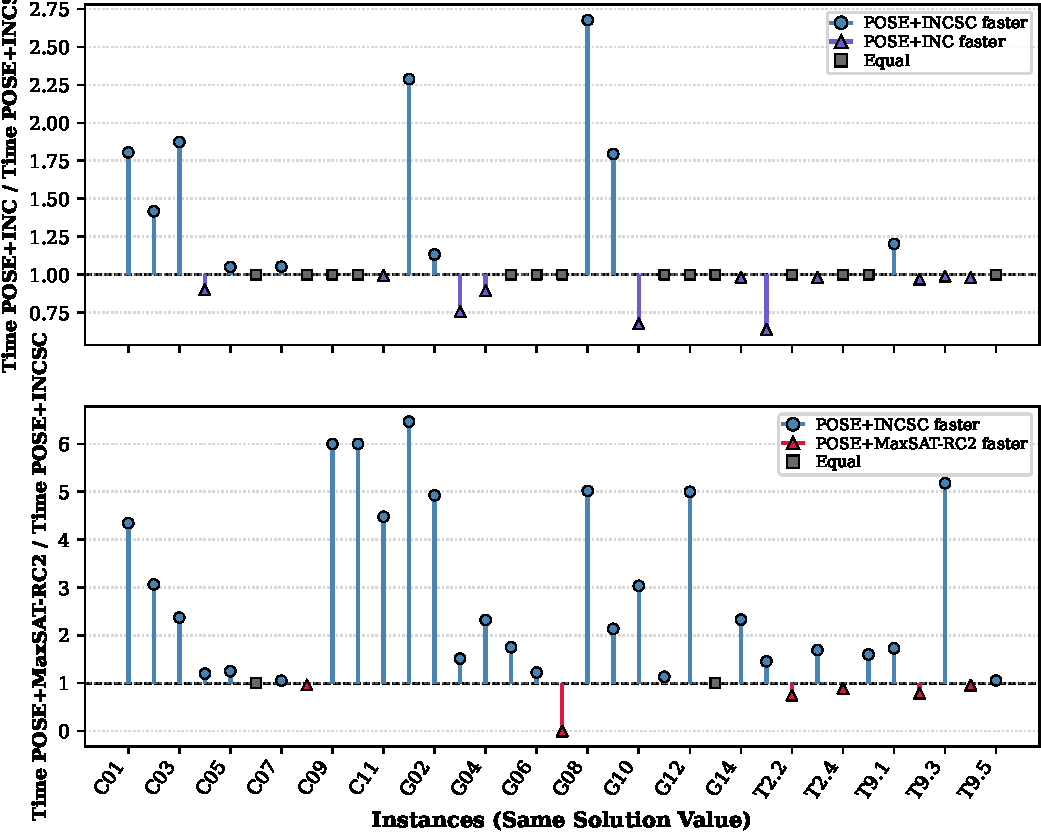
\includegraphics[width=\columnwidth]{image/objective_speedup_lollipop_combined.pdf}
\caption{Time ratio comparison between POSE+INCSC and two objective-function baselines, POSE+INC and POSE+MaxSAT-RC2, on instances with the same reported solution value.}
\label{fig:objective_speedup_lollipop}
\end{figure}

% This acceleration stems from their differing logical topologies. \textbf{INC} uses the \texttt{ITotalizer}'s binary tree \cite{Martins2014Incremental}, which generates numerous auxiliary variables and heavily burdens unit propagation. Conversely, \textbf{INCSC} employs a streamlined Sequential Counter \cite{Sinz2005}. This flat, ``chain-like'' architecture minimizes structural overhead, providing a direct, highly efficient path for Boolean constraint propagation to prune unpromising branches.


\subsection{Comparison with State-of-the-Art Exact Solvers}

% \begin{table*}[!htbp]
% \centering
% \caption{Comprehensive Comparison between Proposed POSE+INCSC and Baseline Methods}
% \setlength{\tabcolsep}{2.5pt}
% \renewcommand{\arraystretch}{1.05}
% \resizebox{\textwidth}{!}{%
% \begin{tabular}{@{}l c ccc ccc ccc ccc ccc ccc ccc@{}}
% \toprule
% \textbf{Inst.} & \textbf{BKS \cite{Gomez2023MO}} & \multicolumn{3}{c}{\textbf{POSE+INCSC}} & \multicolumn{3}{c}{\textbf{POSE+INC}} & \multicolumn{3}{c}{\textbf{DSE+INCSC}} & \multicolumn{3}{c}{\textbf{Gurobi}} & \multicolumn{3}{c}{\textbf{CPLEX-CP}} & \multicolumn{3}{c}{\textbf{CPLEX-MIP}} \\
% \cmidrule(lr){3-5} \cmidrule(lr){6-8} \cmidrule(lr){9-11} \cmidrule(lr){12-14} \cmidrule(lr){15-17} \cmidrule(lr){18-20}
%  &  & \textbf{Sol.} & \textbf{Time} & \textbf{Status} & \textbf{Sol.} & \textbf{Time} & \textbf{Status} & \textbf{Sol.} & \textbf{Time} & \textbf{Status} & \textbf{Sol.} & \textbf{Time} & \textbf{Status} & \textbf{Sol.} & \textbf{Time} & \textbf{Status} & \textbf{Sol.} & \textbf{Time} & \textbf{Status} \\
% \midrule
% C01 & 16 & 16 & \textbf{119.14} & OPT & 16 & 215.06 & OPT & 16 & 600.00 & TO & 20 & 600.00 & TO & 16 & 600.00 & TO & 24 & 600.00 & TO \\
% C02 & 14 & 14 & 9.78 & OPT & 14 & 13.86 & OPT & 14 & 600.00 & TO & 14 & \textbf{7.39} & OPT & 14 & 600.00 & TO & 14 & 600.00 & TO \\
% C03 & 14 & 14 & \textbf{65.31} & OPT & 14 & 122.41 & OPT & 14 & 600.00 & TO & 16 & 600.00 & TO & 14 & 600.00 & TO & 18 & 600.00 & TO \\
% C04 & 46 & 46 & 0.10 & OPT & 46 & 0.09 & OPT & 46 & \textbf{0.07} & OPT & 46 & 0.16 & OPT & 46 & 0.22 & OPT & 46 & 0.12 & OPT \\
% C05 & 40 & 40 & \textbf{0.40} & OPT & 40 & 0.42 & OPT & 40 & 0.79 & OPT & 40 & 1.37 & OPT & 40 & 0.73 & OPT & 40 & 1.10 & OPT \\
% C06 & - & - & \textbf{0.22} & INF & - & \textbf{0.22} & INF & - & 0.49 & INF & - & 0.24 & INF & - & 0.24 & INF & - & 0.23 & INF \\
% C07 & - & - & \textbf{0.19} & INF & - & 0.20 & INF & - & 0.72 & INF & - & 0.20 & INF & - & 0.20 & INF & - & 0.20 & INF \\
% C08 & - & - & \textbf{0.27} & INF & - & \textbf{0.27} & INF & - & 1.73 & INF & - & 0.28 & INF & - & 0.28 & INF & - & \textbf{0.27} & INF \\
% C09 & - & - & \textbf{0.01} & INF & - & \textbf{0.01} & INF & - & 0.02 & INF & - & \textbf{0.01} & INF & - & \textbf{0.01} & INF & - & \textbf{0.01} & INF \\
% C10 & - & - & \textbf{0.01} & INF & - & \textbf{0.01} & INF & - & \textbf{0.01} & INF & - & \textbf{0.01} & INF & - & \textbf{0.01} & INF & - & \textbf{0.01} & INF \\
% C11 & 22 & 22 & 16.49 & OPT & 22 & \textbf{16.42} & OPT & 22 & 600.00 & TO & 22 & 198.57 & OPT & 22 & 600.00 & TO & 32 & 600.00 & TO \\
% G01 & 18 & 18 & 66.73 & OPT & 18 & 152.72 & OPT & 18 & 600.00 & TO & 18 & 5.68 & OPT & 18 & 600.00 & TO & 18 & \textbf{2.19} & OPT \\
% G02 & 14 & 14 & \textbf{14.96} & OPT & 14 & 16.95 & OPT & 14 & 600.00 & TO & 14 & 44.70 & OPT & 14 & 600.00 & TO & 14 & 15.97 & OPT \\
% G03 & 20 & 20 & 5.90 & OPT & 20 & \textbf{4.46} & OPT & 20 & 24.10 & OPT & 22 & 600.00 & TO & 20 & 89.41 & OPT & 32 & 600.00 & TO \\
% G04 & 22 & 22 & 12.21 & OPT & 22 & \textbf{10.93} & OPT & 22 & 58.64 & OPT & 44 & 600.00 & TO & 22 & 315.61 & OPT & - & 600.00 & TO \\
% G05 & - & - & \textbf{0.04} & INF & - & \textbf{0.04} & INF & - & 0.09 & INF & - & \textbf{0.04} & INF & - & \textbf{0.04} & INF & - & \textbf{0.04} & INF \\
% G06 & - & - & \textbf{0.09} & INF & - & \textbf{0.09} & INF & - & 0.49 & INF & - & \textbf{0.09} & INF & - & 0.10 & INF & - & \textbf{0.09} & INF \\
% G07 & - & - & 0.01 & INF & - & 0.01 & INF & - & 0.01 & INF & - & \textbf{0.00} & INF & - & 0.01 & INF & - & \textbf{0.00} & INF \\
% G08 & 18 & 18 & \textbf{38.64} & OPT & 18 & 103.44 & OPT & 18 & 600.00 & TO & 18 & 240.57 & OPT & 18 & 600.00 & TO & 22 & 600.00 & TO \\
% G09 & 18 & 18 & \textbf{159.46} & OPT & 18 & 286.23 & OPT & 18 & 600.00 & TO & 26 & 600.00 & TO & 18 & 600.00 & TO & 28 & 600.00 & TO \\
% G10 & 22 & 22 & 60.55 & OPT & 22 & \textbf{40.94} & OPT & 22 & 600.00 & TO & - & 600.00 & TO & 22 & 600.00 & TO & - & 600.00 & TO \\
% G11 & - & - & \textbf{0.15} & INF & - & \textbf{0.15} & INF & - & 0.98 & INF & - & \textbf{0.15} & INF & - & \textbf{0.15} & INF & - & 0.16 & INF \\
% G12 & - & - & \textbf{0.01} & INF & - & \textbf{0.01} & INF & - & 0.02 & INF & - & \textbf{0.01} & INF & - & \textbf{0.01} & INF & - & \textbf{0.01} & INF \\
% G13 & - & - & \textbf{0.24} & INF & - & \textbf{0.24} & INF & - & 1.45 & INF & - & \textbf{0.24} & INF & - & 0.25 & INF & - & \textbf{0.24} & INF \\
% G14 & 8 & 8 & 8.64 & OPT & 8 & \textbf{8.49} & OPT & 8 & 106.29 & OPT & 8 & 456.71 & OPT & 10 & 600.00 & TO & 16 & 600.00 & TO \\
% T2.1 & 12 & 12 & 2.74 & OPT & 12 & \textbf{1.75} & OPT & 12 & 42.02 & OPT & 12 & 14.22 & OPT & 12 & 600.00 & TO & 12 & 12.34 & OPT \\
% T2.2 & 46 & 46 & \textbf{0.08} & OPT & 46 & \textbf{0.08} & OPT & 46 & 0.26 & OPT & 46 & 0.09 & OPT & 46 & 0.12 & OPT & 46 & 0.09 & OPT \\
% T2.3 & 14 & 14 & 1.13 & OPT & 14 & \textbf{1.11} & OPT & 14 & 8.00 & OPT & 14 & 15.13 & OPT & 14 & 455.48 & OPT & 14 & 345.36 & OPT \\
% T2.4 & 20 & 20 & \textbf{0.09} & OPT & 20 & \textbf{0.09} & OPT & 20 & 0.25 & OPT & 20 & 0.20 & OPT & 20 & 0.16 & OPT & 20 & 0.16 & OPT \\
% T2.5 & - & - & \textbf{0.05} & INF & - & \textbf{0.05} & INF & - & 0.29 & INF & - & \textbf{0.05} & INF & - & \textbf{0.05} & INF & - & \textbf{0.05} & INF \\
% T9.1 & 18 & 18 & \textbf{10.87} & OPT & 18 & 13.07 & OPT & 18 & 58.76 & OPT & - & 600.00 & TO & 22 & 600.00 & TO & 46 & 600.00 & TO \\
% T9.2 & 48 & 48 & 0.34 & OPT & 48 & \textbf{0.33} & OPT & 48 & 0.86 & OPT & 48 & 0.37 & OPT & 48 & 0.48 & OPT & 48 & 0.35 & OPT \\
% T9.3 & 24 & 24 & 4.40 & OPT & 24 & \textbf{4.36} & OPT & 24 & 15.68 & OPT & - & 600.00 & TO & 24 & 35.65 & OPT & 46 & 600.00 & TO \\
% T9.4 & 26 & 26 & 0.51 & OPT & 26 & \textbf{0.50} & OPT & 26 & 1.08 & OPT & 26 & 0.73 & OPT & 26 & 0.79 & OPT & 26 & 0.62 & OPT \\
% T9.5 & - & - & \textbf{0.18} & INF & - & \textbf{0.18} & INF & - & 0.24 & INF & - & 0.19 & INF & - & 0.19 & INF & - & 0.19 & INF \\
% \midrule
% \textbf{Total} & - & - & \textbf{599.94} & - & - & 1015.19 & - & - & 5723.34 & - & - & 5787.40 & - & - & 8100.19 & - & - & 7579.80 & - \\
% \#OPT & - & - & - & \textbf{22} & - & - & \textbf{22} & - & - & 13 & - & - & 14 & - & - & 10 & - & - & 10 \\
% \#INF & - & - & - & 13 & - & - & 13 & - & - & 13 & - & - & 13 & - & - & 13 & - & - & 13 \\
% \#TO & - & - & - & \textbf{0} & - & - & \textbf{0} & - & - & 9 & - & - & 8 & - & - & 12 & - & - & 12 \\
% \bottomrule
% \multicolumn{20}{l}{\footnotesize \textbf{BKS}: Best known solution reported in \cite{Gomez2023MO}; \textbf{OPT}: Optimal; \textbf{INF}: Infeasible; \textbf{TO}: Timeout; \textbf{\#}: Number of instances.}
% \end{tabular}%
% }
% \end{table*}

% Regarding overall convergence, the proposed method successfully solves and mathematically certifies all 35 instances (a 100\% success rate). In stark contrast, the baseline commercial solvers exhibit severe scalability limitations on these densely constrained networks. As evidenced by the early termination of their respective curves in Fig.~\ref{fig:sota_cactus}, CPLEX-CP and CPLEX-MIP solve only 23 instances (65.71\%), timing out (\texttt{TO}) on 12 test cases. Gurobi performs marginally better but still fails on 8 demanding instances (77.14\% success rate). The ability of POSE+INCSC to consistently certify the global optimum (\texttt{OPT}) highlights its profound stability and robustness, particularly on challenging instances (e.g., \texttt{C01}--\texttt{C03}, \texttt{G08}--\texttt{G10}) where commercial solvers become entirely intractable.

% In terms of execution efficiency, Fig.~\ref{fig:sota_cactus} illustrates that the proposed system achieves orders-of-magnitude speedups compared to the baselines. This is most accurately captured by the cumulative execution time across all 35 instances (including penalized 600s timeouts for unresolved cases): POSE+INCSC requires merely 599.94 seconds, whereas Gurobi consumes 5787.40 seconds, and the CPLEX variants exceed 7500 seconds. For heavily constrained topologies such as \texttt{T9.1} and \texttt{T9.3}, commercial solvers exhaust the 600-second limit without conclusive results, whereas POSE+INCSC decisively proves optimality in just 10.87s and 4.40s, respectively. Furthermore, on inherently infeasible (\texttt{INF}) instances, the proposed system is nearly instantaneous (typically under 0.3s). This exceptional performance confirms that the streamlined architecture of POSE successfully empowers the SAT solver's Unit Propagation mechanism, efficiently pruning unpromising branches from the outset with minimal computational overhead.

% Beyond execution speed, the disparity in solution quality upon timeout is critical. Fig.~\ref{fig:solution_quality} isolates the challenging instances where the commercial baselines failed to prove optimality. 
% While CPLEX-CP occasionally found the optimal bound (e.g., \texttt{C01}, \texttt{C03}, \texttt{T9.3}) before timing out, which indicates a bottleneck primarily in the proof phase rather than the search phase, both CPLEX-MIP and Gurobi suffered severe performance degradation.
% For example, on \texttt{T9.1}, CPLEX-MIP returned a sub-optimal bound more than twice as large as the true optimum (46 vs. 18). More problematically, Gurobi completely failed to formulate even a single feasible solution (\texttt{N/A}) for highly constrained networks such as \texttt{G10}, \texttt{T9.1}, and \texttt{T9.3}, and returned heavily sub-optimal allocations for others like \texttt{G09}. Aggregating the solution quality, POSE+INCSC successfully secured and certified all 22 possible optimal solutions, leaving Gurobi (14 \texttt{OPT}) and the CPLEX variants (10 \texttt{OPT} each) significantly behind. These results demonstrate that POSE+INCSC not only scales better but consistently guarantees mathematically optimal allocations where commercial MIP/CP architectures break down.

Finally, POSE+INCSC is compared with Gurobi, CPLEX-CP, CPLEX-MIP, and CP-SAT. Table~\ref{tab:appendix_solver_baselines_preprocess} summarizes these solver results and includes EvalMaxSAT as an additional MaxSAT baseline, while Figs.~\ref{fig:sota_cactus} and~\ref{fig:solution_quality} highlight the differences in solving time and solution quality. 
% For all 22 satisfiable instances, POSE+INCSC matches the Best Known Solutions (BKS) reported in \cite{Gomez2023MO}, supporting the correctness of the proposed exact encoding.
% POSE+INCSC certifies optimality for 22 out of 35 instances, matching the Best Known Solutions (BKS) reported in \cite{Gomez2023MO}. The remaining 13 instances are proven to be infeasible under the considered bounds, further confirming the correctness of the proposed exact encoding.

POSE+INCSC solves and certifies all 35 instances within the 600-second limit, with the longest runtime of approximately 160 seconds (\texttt{G09}). Among the baselines, CP-SAT is the strongest, solving 33 instances and timing out on 2. Gurobi solves 27 instances and times out on 8, whereas CPLEX-CP and CPLEX-MIP solve 23 instances and time out on 12. This gap is also visible in Fig.~\ref{fig:sota_cactus}, where the curve of POSE+INCSC extends further to the right than those of the baseline solvers.
For the 22 satisfiable instances, POSE+INCSC matches the Best Known Solutions (BKS) reported in \cite{Gomez2023MO}, further supporting the correctness of the proposed exact encoding.

\begin{figure}[!htbp]
\centering
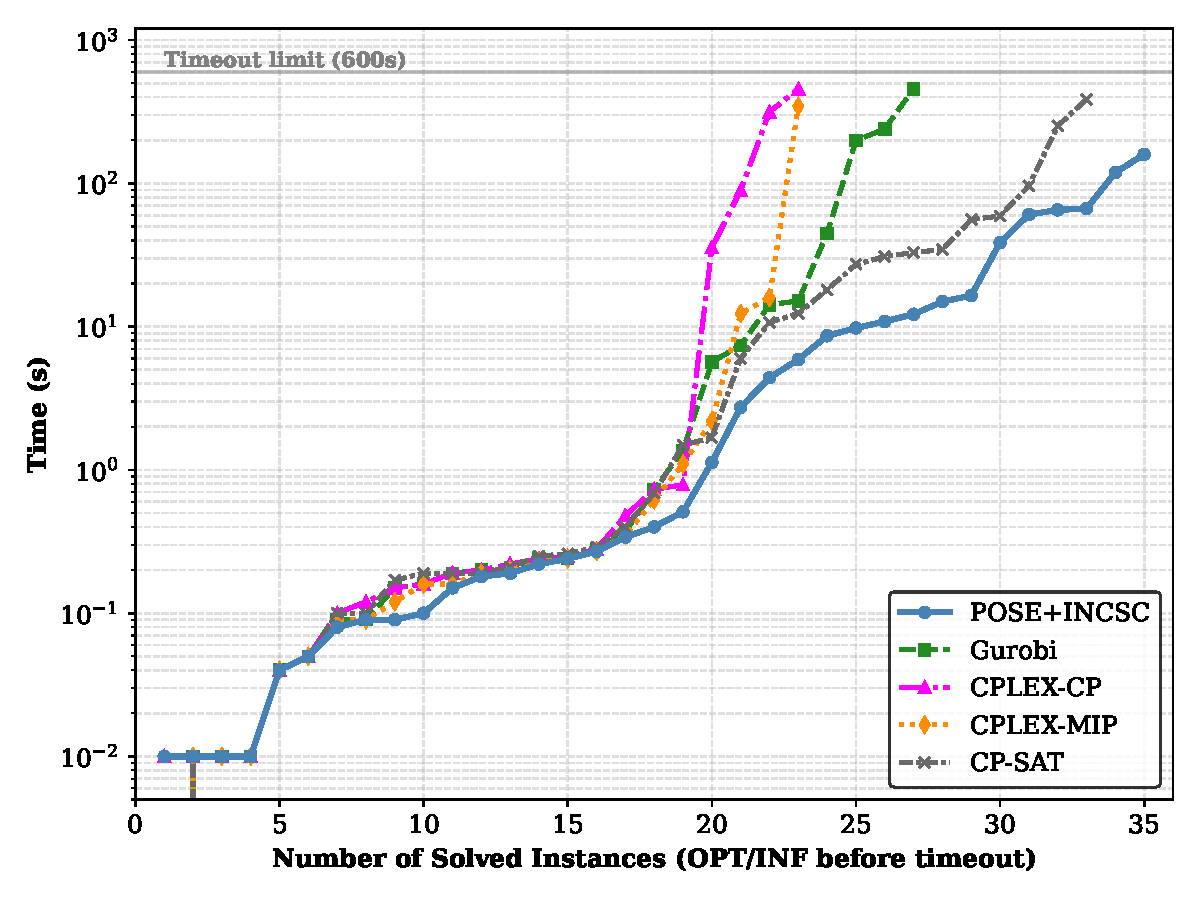
\includegraphics[width=0.95\columnwidth ]{image/sota_cactus_plot.pdf}
% \caption{Cactus plot comparing the overall performance of the proposed POSE+INCSC against Gurobi, CPLEX-CP, and CPLEX-MIP. The x-axis represents the number of successfully solved instances (OPT/INF before timeout), and the y-axis shows the required solving time in a logarithmic scale. A curve extending further to the right and staying lower indicates superior solver performance.}
\caption{Cactus plot comparing the solving time of POSE+INCSC, Gurobi, CPLEX-CP, CPLEX-MIP, and CP-SAT on the 35 benchmark instances.}
\label{fig:sota_cactus}
\end{figure}

\begin{figure}[!htbp]
\centering
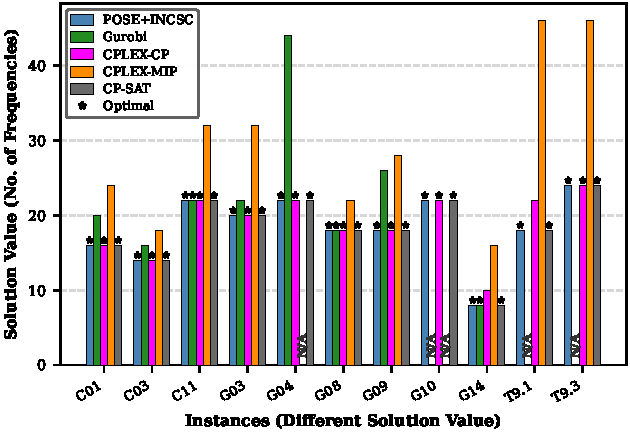
\includegraphics[width=0.95\columnwidth]{image/solution_quality_bar.pdf}
% \caption{Solution quality comparison (objective value) on selected hard instances where baseline commercial solvers exceeded the 600s time limit. Lower values indicate a better solution (fewer frequencies used). Stars ($\star$) denote the optimal value achieved among the shown solvers for that instance. POSE+INCSC consistently achieves optimality in all cases, whereas commercial solvers (Gurobi, CPLEX-CP, CPLEX-MIP) frequently return sub-optimal bounds or fail to find any feasible solution (denoted as N/A) upon timeout.}
\caption{Solution quality comparison on selected hard instances where at least one baseline solver exceeds the time limit or reports a different solution value. Lower values indicate better solutions.}
\label{fig:solution_quality}
\end{figure}

In terms of execution efficiency, POSE+INCSC requires 599.94 seconds of penalized cumulative solving time across all 35 instances, where each timeout is counted as 600 seconds. The corresponding values are 2228.96 seconds for CP-SAT, 5787.40 seconds for Gurobi, and more than 7500 seconds for the CPLEX variants. On difficult cases such as \texttt{T9.1} and \texttt{T9.3}, POSE+INCSC proves optimality in 10.87s and 4.40s, whereas Gurobi, CPLEX-CP, and CPLEX-MIP hit the 600-second limit. CP-SAT is more competitive on these cases but still does not certify all satisfiable instances. On infeasible instances, POSE+INCSC is typically below 0.3s.

The difference in solution quality is most visible on the hard instances where the baseline solvers fail to certify optimality. CP-SAT often finds the same solution value as POSE+INCSC, but it still times out on two satisfiable instances. CPLEX-CP occasionally reaches the optimal bound before timing out (e.g., \texttt{C01}, \texttt{C03}, and \texttt{T9.3}), indicating that its main bottleneck lies in the proof phase. In contrast, CPLEX-MIP and Gurobi often return weaker bounds or no feasible solution at all. For example, on \texttt{T9.1}, CPLEX-MIP returns 46 while the certified optimum is 18, and Gurobi fails to find any feasible solution on instances such as \texttt{G10}, \texttt{T9.1}, and \texttt{T9.3}. Overall, POSE+INCSC certifies all 22 optimal solutions, whereas CP-SAT certifies 20, Gurobi certifies 14, and both CPLEX variants certify 10.



% \begin{table}[!htbp]
% \centering
% \caption{BKS comparison.}
% \label{tab:bks_comparison}
% \scriptsize
% \setlength{\tabcolsep}{4pt}
% \renewcommand{\arraystretch}{1.0}
% \resizebox{\columnwidth}{!}{%
% \begin{tabular}{@{}lccccc@{}}
% \toprule
% \textbf{Inst.} &
% \textbf{BKS \cite{Gomez2023MO}} &
% \textbf{POSE+INCSC} &
% \textbf{Gurobi} &
% \textbf{CPLEX-CP} &
% \textbf{CPLEX-MIP} \\
% \midrule
% C01 & 16 & 16 & 20 & 16 & 24 \\
% C02 & 14 & 14 & 14 & 14 & 14 \\
% C03 & 14 & 14 & 16 & 14 & 18 \\
% C04 & 46 & 46 & 46 & 46 & 46 \\
% C05 & 40 & 40 & 40 & 40 & 40 \\
% C11 & 22 & 22 & 22 & 22 & 32 \\
% G01 & 18 & 18 & 18 & 18 & 18 \\
% G02 & 14 & 14 & 14 & 14 & 14 \\
% G03 & 20 & 20 & 22 & 20 & 32 \\
% G04 & 22 & 22 & 44 & 22 & -- \\
% G08 & 18 & 18 & 18 & 18 & 22 \\
% \bottomrule
% \end{tabular}%
% }
% \vspace{2pt}
% {\footnotesize \textbf{BKS}: Best known solution reported in \cite{Gomez2023MO}.} 
% % ``--'' indicates no feasible solution before timeout.}
% \end{table}


% \begin{table}[!htbp]
% \centering
% \caption{Overall summary of solver performance on the 35 benchmark instances.}
% \label{tab:solver_summary}
% \footnotesize
% \setlength{\tabcolsep}{4.5pt}
% \begin{tabular}{@{}lrrrr@{}}
% \toprule
% \textbf{Method} & \textbf{\#OPT} & \textbf{\#INF} & \textbf{\#TO} & \textbf{Total Time (s)} \\
% \midrule
% POSE+INCSC & 22 & 13 & 0  & \textbf{599.94} \\
% POSE+INC   & 22 & 13 & 0  & 1015.19 \\
% DSE+INCSC  & 13 & 13 & 9  & 5723.34 \\
% Gurobi     & 14 & 13 & 8  & 5787.40 \\
% CPLEX-CP   & 10 & 13 & 12 & 8100.19 \\
% CPLEX-MIP  & 10 & 13 & 12 & 7579.80 \\
% \bottomrule
% \end{tabular}
% \end{table}

\input{../SourceCode/visualize/tables/appendix_sat_core_preprocess.tex}
\input{../SourceCode/visualize/tables/appendix_solver_baselines_preprocess.tex}

\section{Conclusion}
\label{sec:conclusion}
% This paper presents an exact SAT-based framework for solving and certifying optimality in the Minimum Order Frequency Assignment Problem (MO-FAP). The proposed approach is built upon two main components. First, the order-based SAT encoding (POSE) transforms pairwise interference constraints into compact interval-based logical constraints, significantly reducing the size of the search space. Second, the incremental SAT strategy (INCSC), based on Sequential Counter encoding and assumptions, enables efficient reuse of learned clauses across iterations without reconstructing the formula.
This paper presents an exact SAT-based framework for solving and certifying optimality in the MO-FAP. The proposed approach is built upon two main components. First, the order-based SAT encoding (POSE) uses standard order variables together with a problem-specific interval-boundary formulation to replace many pairwise interference conflicts of the direct SAT encoding. Second, the incremental SAT solving strategy (INCSC), based on Sequential Counter encoding, enables efficient reuse of learned clauses across iterations without reconstructing the formula.
% Experimental results on standard benchmark instances show that the proposed POSE+INCSC framework can reliably certify optimality for all tested cases, while consistently outperforming state-of-the-art commercial solvers in both solution time and optimality certification. These findings indicate that the proposed SAT-based approach provides an effective and robust alternative to traditional optimization methods.
Empirical evaluations on the 35 tested benchmark instances show that the proposed SAT-based framework certifies optimality or infeasibility for all instances within a 600-second time limit. Compared to the direct SAT encoding, POSE+INCSC reduces the penalized cumulative execution time by approximately 89.52\% under this evaluation protocol. Furthermore, on this benchmark set and under the reported settings, the proposed framework achieves lower cumulative runtime than the considered commercial exact solvers, particularly on highly constrained instances.
These results support the effectiveness of the proposed SAT-based architecture as an exact method for the tested MO-FAP benchmarks.
% Future work will focus on extending the proposed framework to other FAP variants, such as MS-FAP and MI-FAP, and investigating hybrid strategies that combine SAT solving with metaheuristic techniques to further improve scalability for large-scale communication networks.
% Future research will focus on extending this framework to other FAP variants and real world dataset of MO-FAP. Additionally, we aim to investigate hybrid strategies that integrate SAT-based exact solving with metaheuristic techniques to further enhance scalability for large-scale communication networks.
Future work will extend the proposed framework to other FAP variants and real-world MO-FAP datasets. We also plan to investigate hybrid approaches that combine SAT-based exact solving with metaheuristic methods to improve scalability on large-scale communication networks.

\section*{Data and Code Availability}
\label{sec:data_code_availability}
The source code and benchmark data used in this study are publicly available at: \url{https://github.com/dev2points/Min-Order-Frequency-Assignment-Problem}.

% \appendices

% \balance
% \enlargethispage{2\baselineskip}
\bibliographystyle{IEEEtran}
\bibliography{reference}
% \vfill\eject
% \begin{IEEEbiography}[{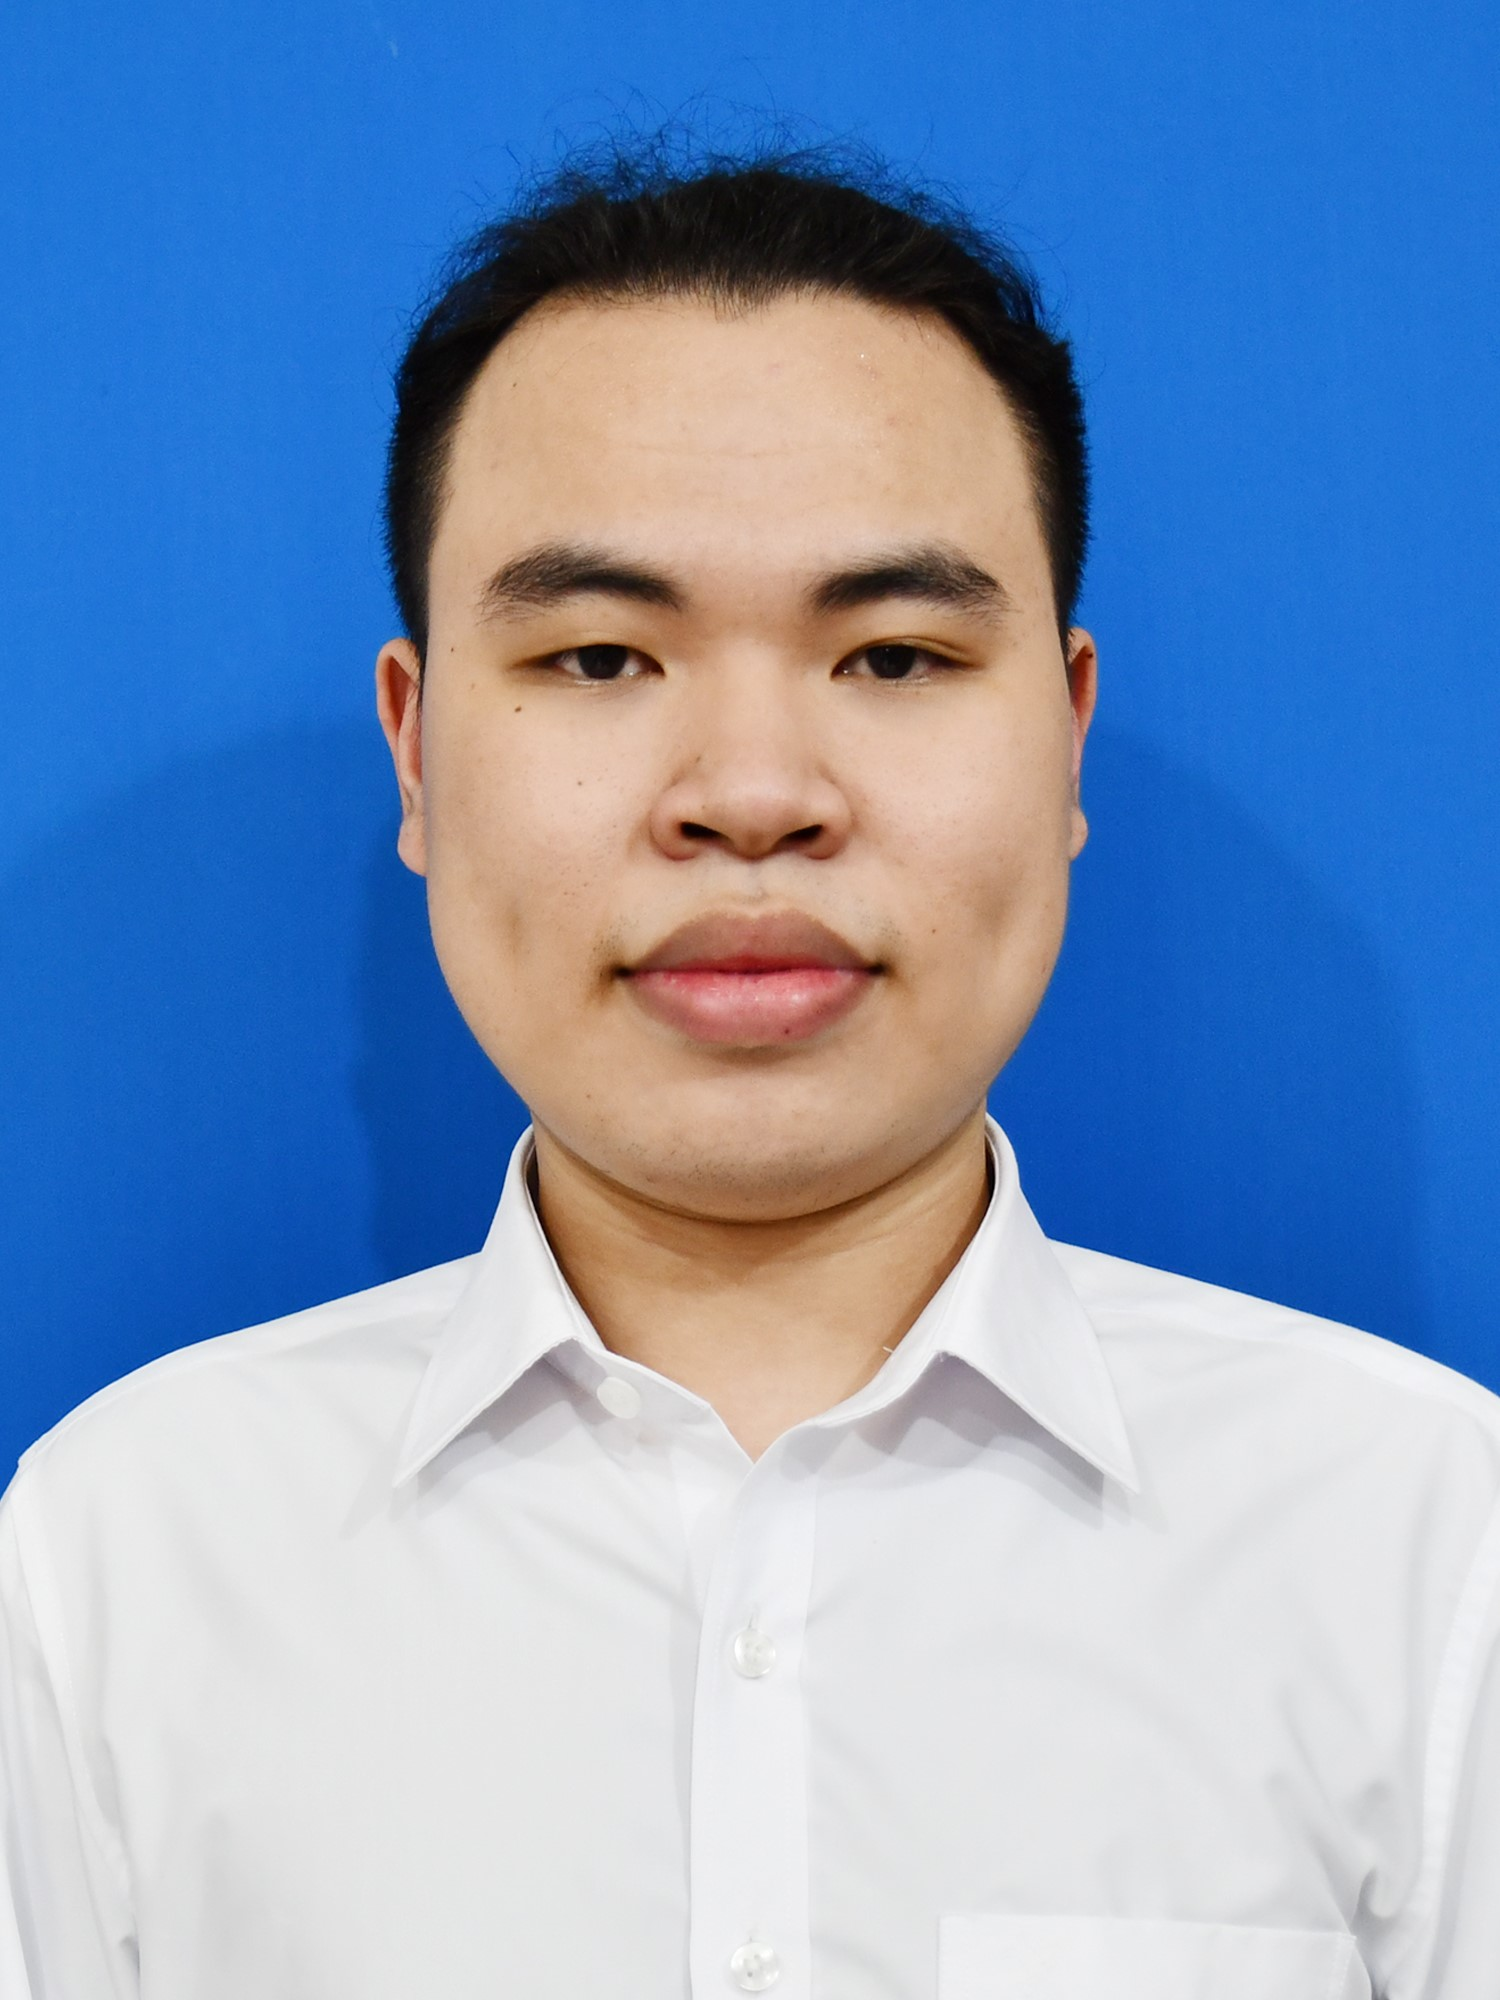
\includegraphics[width=1in,height=1.25in,clip,keepaspectratio]{image/Nghia_Dao_Xuan.jpg}}]{Nghia Dao Xuan} 
% received the B.Sc. degree in Computer Science from the University of Engineering and Technology, Vietnam National University, Hanoi, Vietnam. He is currently pursuing the M.Sc. degree at VNU-UET. His primary research interests include combinatorial optimization, Boolean Satisfiability (SAT), and resource allocation in telecommunication networks.
% \end{IEEEbiography}
% \begin{IEEEbiography}[{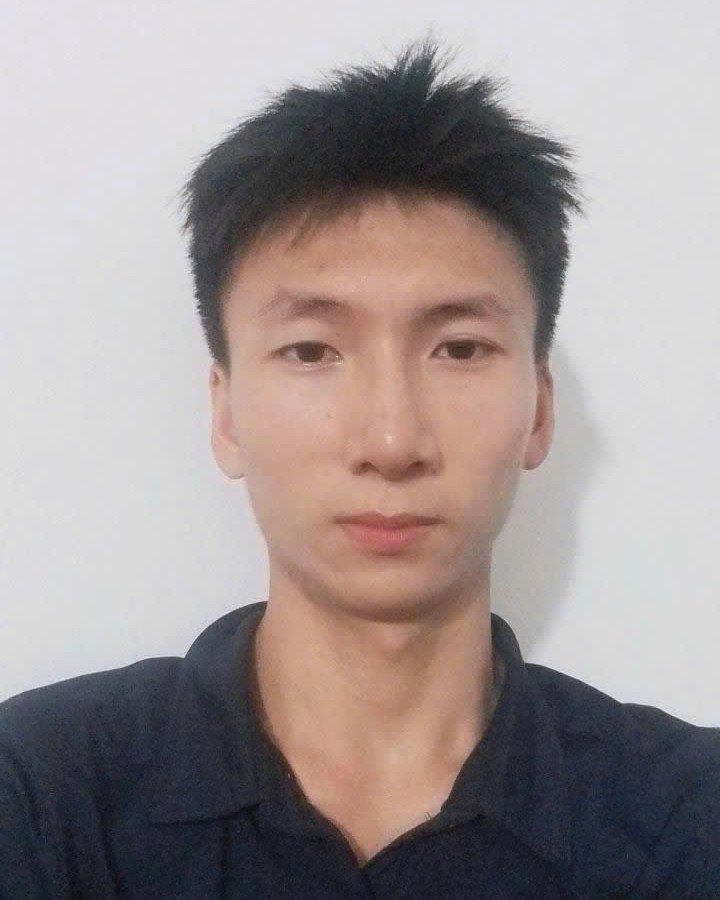
\includegraphics[width=1in,height=1.25in,clip,keepaspectratio]{image/Phuong_Dang_Anh.jpg}}]{Phuong Dang Anh}
% is currently an undergraduate student in information technology at University of Engineering and Technology, Vietnam National University, Hanoi, Vietnam. His research interests include combinatorial optimization, SAT-based methods, and applications of exact solving techniques in discrete optimization problems.
% \end{IEEEbiography}
% \begin{IEEEbiography}[{
\includegraphics[width=1in,height=1.25in,clip,keepaspectratio]{image/Khanh_To_Van.jpg}}]{Khanh To Van}
% received the B.Sc. and M.Sc. degrees from the University of Engineering and Technology, Vietnam National University, Hanoi, Vietnam, in 2004 and 2007, respectively. He earned the Ph.D. degree in Information Science from the Japan Advanced Institute of Science and Technology (JAIST), Ishikawa, Japan, in 2013, where his doctoral research focused on SAT and SMT solving. His research interests include formal methods in software engineering and the development of efficient logical encodings for combinatorial optimization and operations research problems, with a particular emphasis on SAT solving.
% \end{IEEEbiography}

% \vfill
% \enlargethispage{2\baselineskip}
\begin{IEEEbiography}[{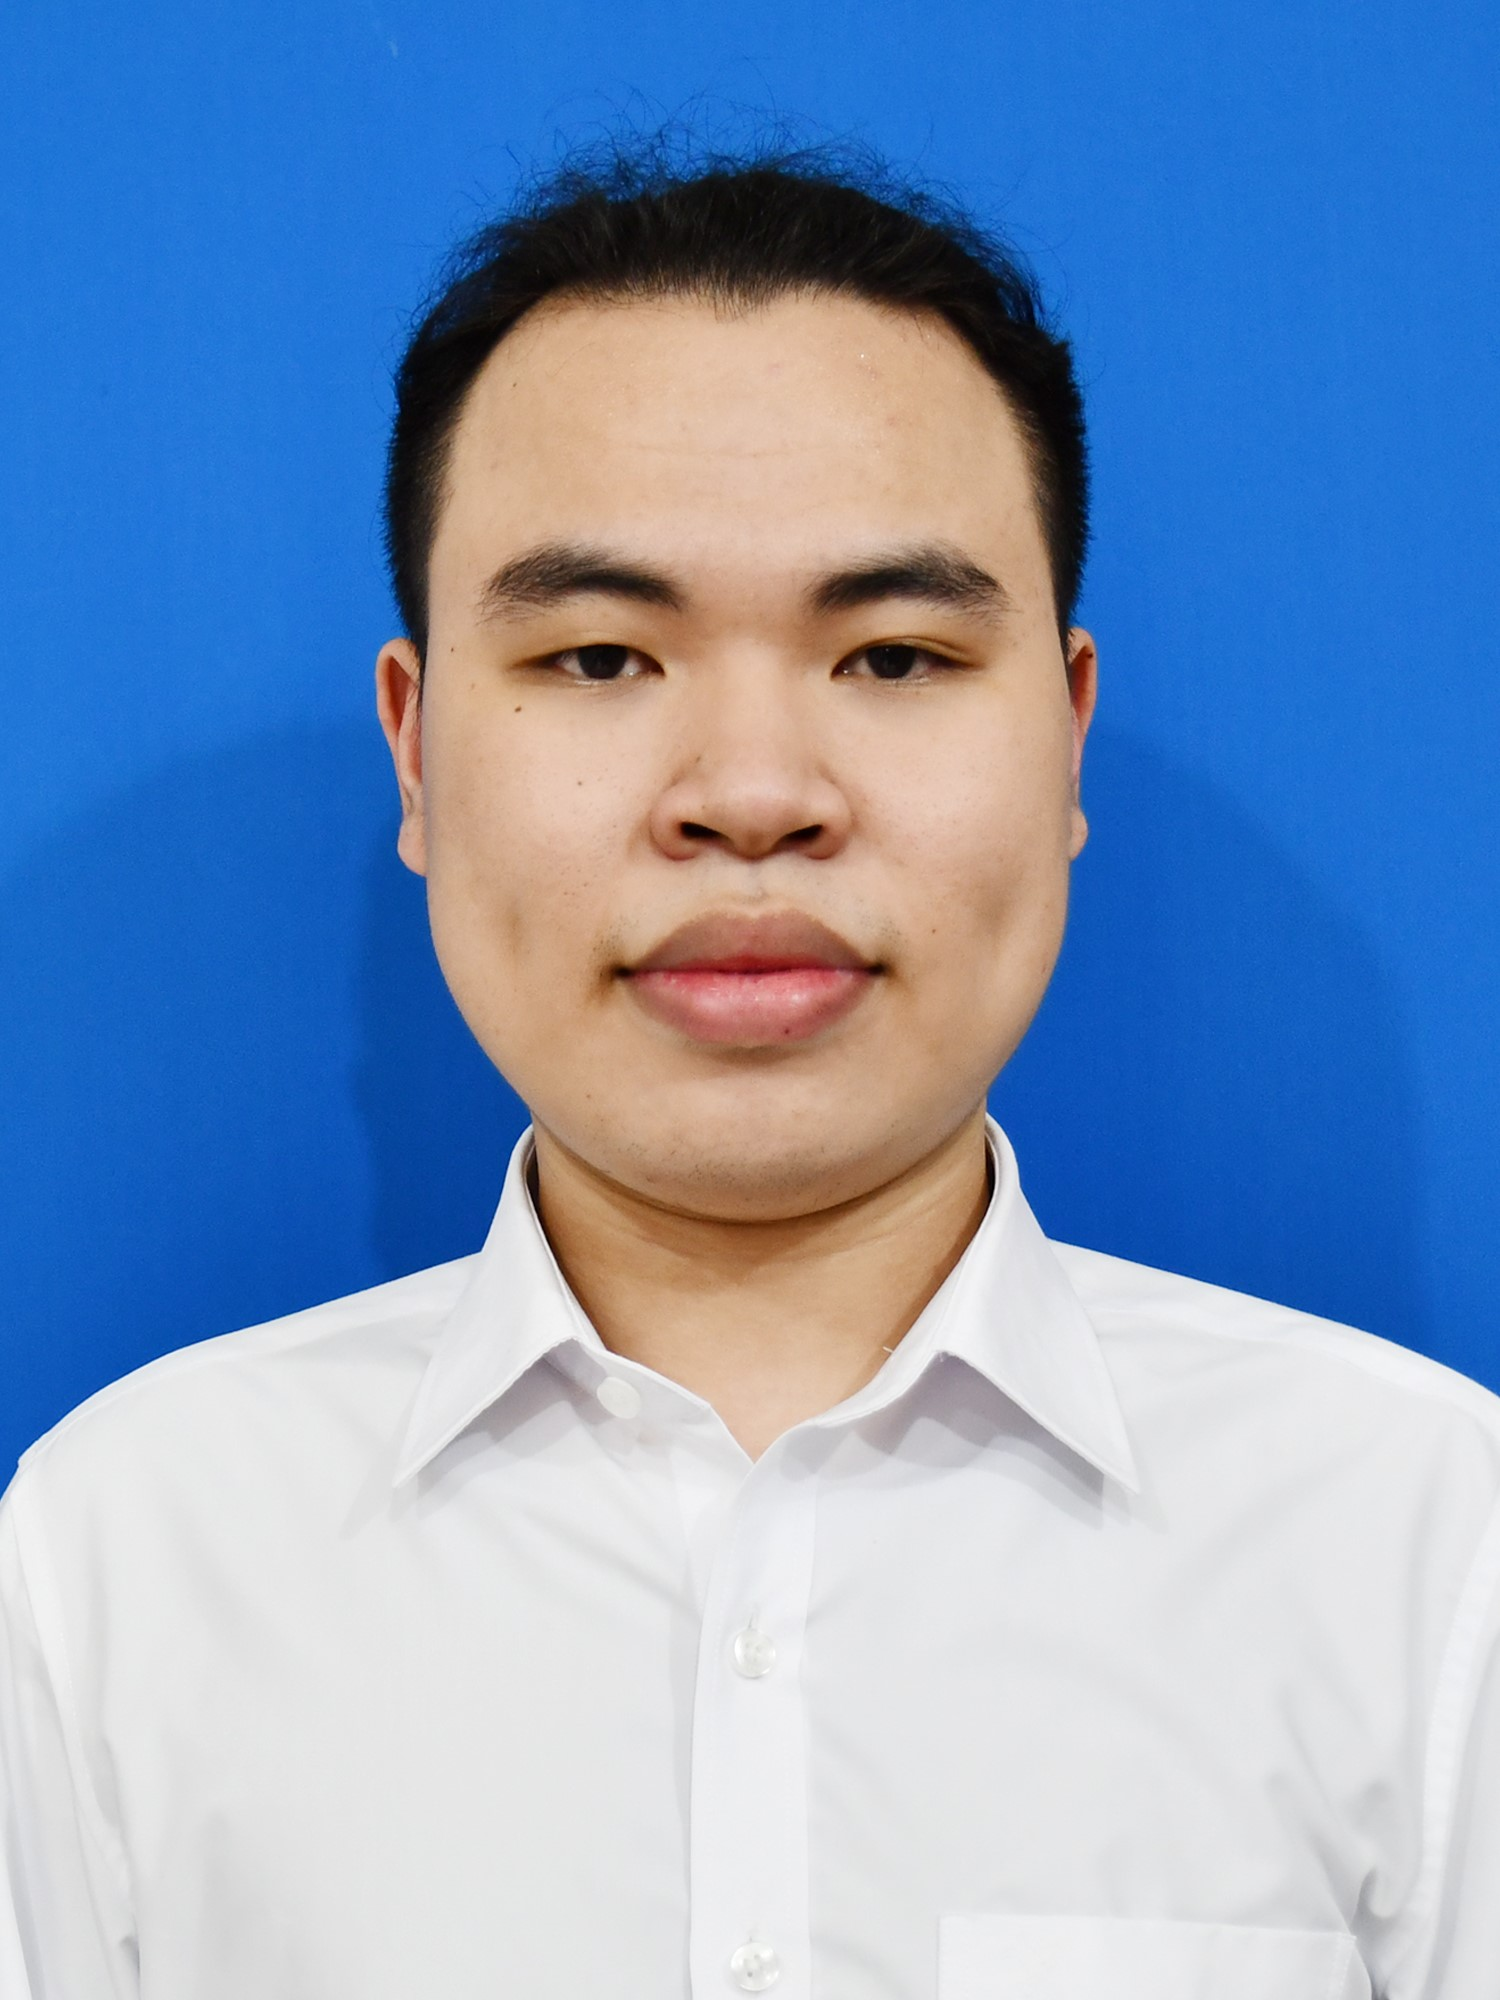
\includegraphics[width=1in,height=1.25in,clip,keepaspectratio]{image/Nghia_Dao_Xuan.jpg}}]{Nghia Dao Xuan}
received the B.Sc. degree in computer science from VNU University of Engineering and Technology, Hanoi, Vietnam, where he is currently pursuing the M.Sc. degree. His research interests include combinatorial optimization, SAT, and telecommunication resource allocation.
\end{IEEEbiography}
\begin{IEEEbiography}[{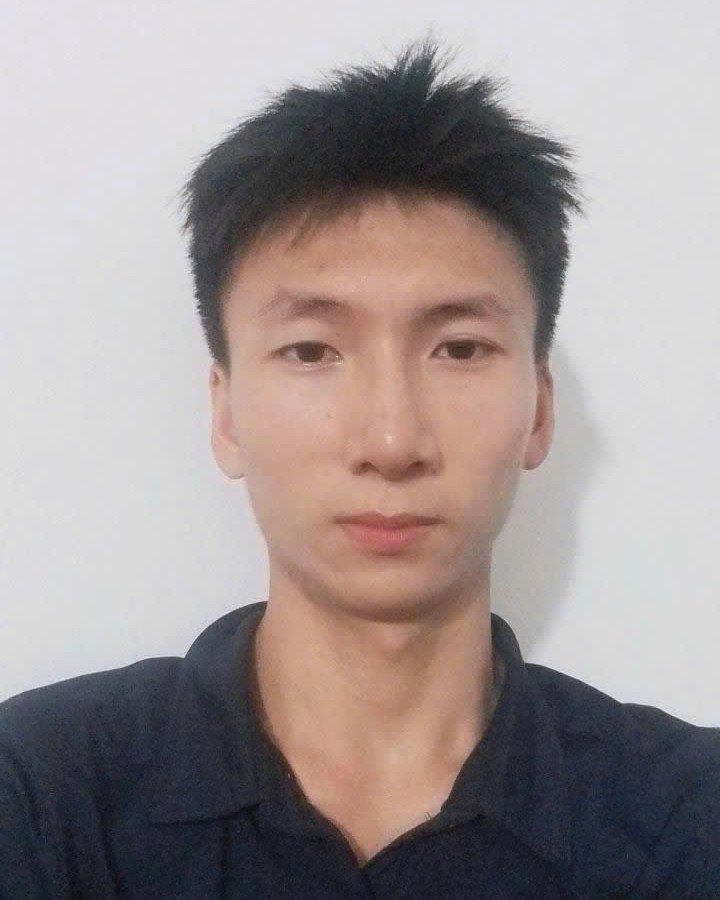
\includegraphics[width=1in,height=1.25in,clip,keepaspectratio]{image/Phuong_Dang_Anh.jpg}}]{Phuong Dang Anh}
is an undergraduate student in information technology at VNU University of Engineering and Technology, Hanoi, Vietnam. His research interests include combinatorial optimization and SAT-based exact methods.
\end{IEEEbiography}
\begin{IEEEbiography}[{
\includegraphics[width=1in,height=1.25in,clip,keepaspectratio]{image/Khanh_To_Van.jpg}}]{Khanh To Van}
received the B.Sc. and M.Sc. degrees from the University of Engineering and Technology, Vietnam National University, Hanoi, Vietnam, in 2004 and 2007, respectively. He earned the Ph.D. degree in Information Science from the Japan Advanced Institute of Science and Technology (JAIST), Ishikawa, Japan, in 2013, where his doctoral research focused on SAT and SMT solving. His research interests include formal methods in software engineering and the development of efficient logical encodings for combinatorial optimization and operations research problems, with a particular emphasis on SAT solving.
\end{IEEEbiography}

\vfill
\end{document}
